% \documentclass[preprint,review,12pt,3p,authoryear]{elsarticle}
\documentclass[preprint,review, 11pt,3p,authoryear]{elsarticle}

\graphicspath{ {./figs/} }
\usepackage{units}
\usepackage{amsmath}
\usepackage{amssymb}
\usepackage[utf8]{inputenc} % set input encoding (not needed with XeLaTeX)
\usepackage[linesnumbered,ruled,vlined]{algorithm2e}

\usepackage{graphicx}

%\usepackage{supertabular}
%\usepackage[sort&compress,round,comma,numbers]{natbib}
\usepackage{graphicx} % support the 
\usepackage{array} % for better arrays (eg matrices) in maths
\usepackage{paralist} % very flexible & customisable lists (eg. enumerate/itemize, etc.)
\usepackage{verbatim} % adds environment for commenting out blocks of text & for better verbatim
% These packages are all incorporated in the memoir class to one degree or another...
\usepackage{booktabs, multicol, multirow,longtable}
\usepackage{tabularx}% http://ctan.org/pkg/tabularx
\usepackage{pdflscape}
\setlength\tabcolsep{3pt}
\usepackage{url}
\urlstyle{same}
\usepackage{threeparttable}
\def\bibsection{\section*{References}}
\usepackage{subfig}
\PassOptionsToPackage{hyphens}{url}\usepackage{hyperref}
\usepackage{color}
\usepackage[dvipsnames]{xcolor}
\usepackage{setspace}
\usepackage{lscape}
\usepackage{subcaption}

\usepackage{floatrow}
\floatsetup[table]{capposition=top}
\usepackage{float}
\restylefloat{table}
\usepackage{mathrsfs}
\usepackage{amsfonts}


\usepackage{algorithm,algorithmic}





\usepackage{bm} % use \pmb for bold in math
\usepackage{gensymb}
\graphicspath{ {figs/} }
\usepackage{lineno}
\usepackage[normalem]{ulem}

\newcommand{\rev}{\color{black}} %% revision blue

\usepackage{float}
\floatstyle{plaintop}
\restylefloat{table}


\journal{journal Name}

\begin{document}
\begin{frontmatter}
\title{Digital Twins: A Simulation-Based and Multi-Objective Realtime Stochastic Approach for Fighting Wildfires}



% ADDITIONAL NOTES!
% GOOD PROJECTS!
% https://tomekent.com/publication/kent-2019/



%% Group authors per affiliation:
% \author{Mohammad Ramshani}
% \author{Xueping Li\corref{mycorrespondingauthor}}
% \author{Anahita Khojandi}
% \author{Olufemi Omitaomu}
% \address{Radarweg 29, Amsterdam}
% \fntext[myfootnote]{Since 1880.}

%% or include affiliations in footnotes:
% \author[mymainaddress]{Mohammad Ramshani}
% \author[mymainaddress]{Jim Ostrowski}
\author[mymainaddress]{Jose Tupayachi}
% \author[mymainaddress]{Xueping Li\corref{mycorrespondingauthor}}
% \ead{xueping.li@utk.edu}
% \author[mymainaddress]{Kaike Zhang}
%\author[mymainaddress,mysecondaryaddress]{Olufemi Omitaomu}
%\author[mythirdaddress]{Jon~Michael Hathaway}
%\ead[url]{www.elsevier.com}

% \author[mysecondaryaddress]{Xueping Li\corref{mycorrespondingauthor}}
% \cortext[mycorrespondingauthor]{Corresponding author}
% %\ead{support@elsevier.com}

\address[mymainaddress]{Department of Industrial and Systems Engineering, The University of Tennessee at Knoxville, Knoxville, TN 37996, US}
% \address[mysecondaryaddress]{Urban Dynamics Institute, Oak Ridge National Laboratory, Oak Ridge, Tennessee 37831, US}
% \address[mythirdaddress]{Department of Civil and Environmental Engineering, The University of Tennessee at Knoxville, Knoxville, TN 37996, US} 


\doublespacing

\begin{abstract}
Worldwide, ecosystems, communities, and economies are under increased threat from wildfires. Micro Aerial Vehicles (MAVs) and agent-based modeling offer a dynamic method for detecting, preventing, and responding to wildfires. We investigate the potential collaboration between agent-based simulation and MAVs in addressing the dynamic challenges of wildfire management.
Simulation considers weather, geography, and vegetation, agent-based simulation augments real-time data by the inclusion of wildfire-prone locations. The spread of the fire and locating high-risk regions, to shifting wildfire conditions and help with resource allocation and decision-making. MAVs and agent-based simulation work together to provide a comprehensive strategy to managing and detecting wildfires. The model's situational awareness is improved by including real-world MAV data, which also helps to identify ignition sources and forecast the direction and rate of a fire. We highlight the ability to lessen the effects of wildfires by providing information on how to allocate resources, make evacuation plans, and prepare communities.

% Uncapacitated facility location problems ({\rev {UFLPs}}) deal with the selection of facilities and assignment of customers to them. Two level UFLPs ({\rev {TUFLPs}}) consider an additional level of facilities between the customers and the main facilities, through which the customers are connected to the production facilities. Disruption uncertainty introduces more complexity to such problems as it accounts for the probability that facilities may not always be able to satisfy the demand of their assigned customers. In this paper, we study a TUFLP with single assignment under disruption uncertainty. We investigate a two-level distribution chain, in which the flow starts from the production unit, goes through distribution centers, and then ends at the customer level. We assume a region based single commodity distribution chain whose components, excluding the customers, are prone to breakdowns due to disasters. We develop two mathematical programming formulations for the problem and develop a Tabu search algorithm and a problem specific heuristic (route subset selector - RSS), and interpret the results.
%Therefore, the disruption matrix includes a covariance of disruptions where components in the same region are more likely to be shut down at the same time.
\end{abstract}

\begin{keyword}
MAVs, CVRP, Agent Based Simulation, Discrete Simulation, Wildfires
%stochastic programming\sep Photovoltaic panels\sep climate change\sep energy saving\sep green roofs
\end{keyword}

\end{frontmatter}

% \modulolinenumbers[5]
% \linenumbers

\section{Introduction}
\label{intro}

Wildfires are one of the most expensive and deadly natural catastrophes in the world, particularly in the western United States. In 2018, a catastrophic wildfire known as the Camp Fire was recorded as one of the worst wildfires in the history of California. 
Yet these catastrophic fires are expected increase by the year 2050 \cite{united_nations} if preventive actions are not taken nor improvement of response services are studied. These fire events are responsible of large-scale evacuation, homes being set on fire, infrastructure being destroyed, millions of hectares of forest resources damaged, and most critically, human lives being in danger.
Fire detection and monitoring technologies have evidenced an rapid increase such as ground sensors, Unmaned Aerial Vehicle (UAVs), and satellite imagery have been deployed.
Current systems have the following drawbacks which include delayed fire detection due to missing minor fires in the early stages, relatively high time lag for satellites to overhead the field, and inability to deploy sensors with restricted detecting distance ranges. For instance, a prompt response is desirable as they are likely to put off fire events on the early stages. It is demmed reponse times and proper resource allocation are key components for a prompt and adequated response.
% This study aims to capitalize on the potential of FPV lightweight micro-air vehicles (MAVs),  outfitted with advanced high-resolution cameras and an integrated communication system to proactively detect and monitor activities of interest (AOIs) in a busy metropolitan area." Our major goal is to create a network of aerial MAVs that is seamlessly integrated, establishing a dynamic mesh system. This novel technique answers the demand for effective and comprehensive metropolitan monitoring. We build a collaborative system in which MAVs may interact with one another, share information, and work together to cover a bigger area more effectively by joining these MAVs in a mesh network. We denote mesh system to the join work 
% Fast detection of AOIs in the POIs located in certain geographical areas partitioned by quadrants is possible with FPV MAVs. We use cutting-edge Machine Learning techniques, notably computer vision algorithms, to allow autonomous AOI detection. These algorithms enable our MAVs to recognize and categorize AOIs autonomously, minimizing the need for user involvement and shortening reaction times. Each MAV in the mesh network is capable of transmitting to report AOIs to a centralized server using the embedded communication system, ensuring a dispersed and coordinated monitoring effort. Furthermore, we use evolutionary algorithms to improve MAV routing inside the mesh system, based on a multiple traveling salesman problem (mTSP) guaranteeing effective resource allocation and rapid reaction to discovered AOIs. This implies that the MAVs may alter their placements and routes dynamically to give optimal coverage and reaction times. Our research goes beyond the creation of hardware and algorithms, as well. We replicate and carefully examine the dispatch and service activities of emergency response teams using discrete event modeling. Our linked MAV mesh system's efficacy and operating dynamics are better understood as a result, and this highlights the system's importance for expediting emergency response operations and enhancing overall urban safety.
On the basis of these we center our research effort on a proper allocation of resources and simulation of fire events course of action through the use of optimization based agent based simulation.
This study aims to capitalize the use of the listed techniques to propose a practical framework for fire events hadling and resource allocaiton in the context of wildfires using a set of heterogeneous agents drones to provide adequate responses when human controllers are not available to initiate and guide the mission.




% Facility location problems ({\rev{FLPs}}) are mainly studied to choose the best facility locations in order to {\rev{optimize}} various objectives, e.g., total travel time, total transportation cost, total annual operating cost, total setup cost, and physical distance \citep{farahani2014hierarchical}. There is a rich body of literature which focuses on the development of different types of FLPs \citep{drezner2001facility,eiselt2011foundations,laporte2015location,daskin2011network}.

% FLPs are often studied with the assumption of no capacity restriction over the facilities, i.e., uncapacitated problems {\rev{\citep{cornuejols1983uncapacitated,kuehn1963heuristic,kratica2014new,hakli2019improved}}}. 
% %, whereas a number of studies have taken a different approach and set capacity restrictions on the facilities, i.e., capacitated problems \citep{aardal1995capacitated,aardal1998reformulation}. Both capacitated and uncapacitated FLP problems have been studied considering different assumptions on the number of facility levels, i.e., single-level \citep{byrka2007optimal,jakob1983simple,francis1983locational,erlenkotter1978dual} where the objective is mainly to decide where to locate a facility and which customers should be assigned to each open facility, and multi-level \citep{ortiz2017multi,kratica2014new,ortiz2017multi} where the objective to serve each customer with a sequence of facilities. 
% {\rev{In uncapacitated FLPs (UFLPs)}}, facilities are selected from a finite set of potential sites, and each customer from a finite set of customers with known respective demand is assigned to one of the located facilities in order to {\rev {optimize}} the total transportation costs, i.e., a $p$-median model. The total costs subjected to minimization in some models also include the facility opening cost, i.e., fixed-charge models \citep{gendron2016lagrangian}.
% The two level uncapacitated facility locationing problem (TUFLP), which is considered as an extension of the UFLP \citep{gendron2016lagrangian}, was first introduced by \cite{kaufman1977plant} in the  seminal article ``A plant and warehouse location problem''.
% %in which the authors aimed to simultaneously determine the best locations for two sets of facilities and warehouses. 
% In TUFLP, there exists two levels of potential facility locations, which are often addressed as ``depots'', for the higher level facilities, and ``satellites'', for the lower level facilities \citep{gendron2016lagrangian}. {\rev{TUFLPs}}  mainly consider that the products can be shipped only between two consecutive levels, e.g., depots and satellites, or satellites and customers. 
% The objective of TUFLPs is to decide which depots and satellites to open, and to which pair of depots and satellites each customer should be assigned, in order to minimize the total costs \citep{aardal1996two}, through which the flow of the products between each two stages is determined. 
% %This problem is mostly studied in 
% %and it was extended to multi-level UFLPs (MUFLP) [Aardal, Chudak, and Shmoys (1999)], the authors extended the TUFLP problem into multi-level UFLP (MUFLP).
% %TUFLP models have been studied in a variety of areas of application such as freight transportation [CITE-BASE Gendron], and telecommunication [BASE-Chardaire]. 
% {\color{black}TUFLP is widely studied in the literature, such as proposing heuristic solution procedures to jointly locate central and regional distribution centers \citep{gao1992dual}, developing a branch and bound algorithm to solve mixed integer linear programming (MILP) model with a fixed-charge objective function \citep{barros1992general}{\rev{, and studying multi-level UFLPs with a focus on selecting the routes between each level of facilities \citep{ortiz2019exact}.}}

% %For example, \cite{gao1992dual} propose a dual-based heuristic solution procedure for a TUFLP to jointly locate central and regional distribution centers. The proposed solution procedure is an extension to the dual ascent and adjustment procedure for UFLP problems \citep{erlenkotter1978dual} which provides a tight lower bound to be used as a heuristic solution approach or to be incorporated in branch-and-bound algorithms. They examine the solution procedure over 420 test problems, the largest of which considers 25 potential facility locations along with 35 customer sites, and conclude that over 72\% of the test problems achieve the optimal solution without the incorporation of any branch-and-bound algorithms. In another study, \cite{barros1992general} propose a mixed integer linear programing (MILP) model with a fixed-charge objective function, and solve the model by developing a Lagrangian relaxation based branch and bound algorithm. 
% %In another study, \cite{gendron2017comparison} propose six MILP models for TUFLP with single assignment through implementation of reformulation methods and the relaxation of integrality of location variables. The developed MILP models differ in the way that they impose the single assignment constraint in which the weak models only consider the depot-satellite assignment variables whereas the strong models consider a tight connection between the depot-satellite assignment variables and the satellite location variables. The models are theoretically and computationally examined by solving a number of hypothetical and real life instances for freight transportation. Their results show that for the cases when the installation costs of depots (satellites) are significant the best practice is to maintain the integrality of their corresponding variables while the integrality of the binary variables related to satellites (depots) is relaxed. Moreover, the formulations in which the number of binary variables are minimized, through the relaxation of binary variables of the both types of location variables, yield poor results. The authors also conclude that cases in which the costs for satellites are high are the most difficult problems to solve.

% %The structural behavior of TUFLP problems has also been the subject of a number of studies. For example, \cite{aardal1996two} investigate the structural properties of TUFLP problems. First, they present two multi-commodity TUFLP models and study the relationship between them and UFLPs. Then, they show that all nontrivial facets for UFLP problems also define facets for the two-level models, and derive conditions under which the facets for UFLP problems are also the facets for the two-level problem. %In another study, [] introduce a new class of ``dicut collection'' inequalities, and show that these constraints completely describe the projection of the multi-commodity formulation onto original variables.  



% %2 https://pdfs.semanticscholar.org/c337/725332126f32a2e3b484f3432dde7abc03b8.pdf

% %The vast utilization of just-in-time and lean production philosophies as well as globalization has made supply chains more dependent on the availability of their components, of which facilities are the most crucial. 

% {\color{black}Single assignment constraints impose additional restrictions on TUFLP models. Through single assignment constraints, model ensures that each level is supplied only by one facility on their previous level. That is, each customer is supplied only through one satellite, while each satellite is supplied only by one depot. These single assignment constraints appear in a number of applications in the literature.} {\rev{For example, \citet{gendron2017comparison} applied the single assignment constraints in six different reformulations of TUFLP, and evaluated them using artificial and real world problems. In another study, \cite{gendron2015multilayer} proposed a single assignment TUFLP model and used a variable neighborhood search (VNS) meta-heuristic method to solve the proposed model over 90 test problems for the classical TUFLPS, and a real-life problem with modular costs.}}


% %For example, \cite{gendron2015multilayer} propose a single assignment TUFLP model and developed a multilayer variable neighborhood search (VNS) meta-heuristic method to solve the proposed model. This method partitions the neighborhood structures into multiple layers in order to perform a VNS on each layer separately while the whole process in recursively evaluated by the multilayer VNS method. They evaluate their proposed method through its performance over 90 test problems for the classical TUFLPS, and a real-life problem with modular costs. The authors conclude that the results from the test problems show the quality of the lower bounds obtained for path-based integer programming formulations.
% %In another study, \cite{chardaire1999upper} propose a TUFLPS in the telecommunications industry, for a concentrator access network. They propose two different formulations for the problem, i.e., a simple plant location problem and an improved version of the same model with more variables included. The authors develop a simulated annealing algorithm to provide solutions for the first model, while incorporating facet defining cuts as well as well as providing a Lagrangian relaxation for the improved version of the model. They further show that the linear relaxation of the two model formulations result in the same optimal solution, evaluate the solution methods, and provide insights. 

% In the classical {\rev{UFLP and TUFLP}}, it is assumed that once the facilities are setup, they are always available. However, in reality the facilities may become unavailable due to a variety of reasons ranging from natural disasters, such as earthquake or flood, to human actions, such as terrorist or cyber attacks, or change of the ownership \citep{snyder2005reliability,snyder2016or}.

% Facility failures and disruption in supply chain are not frequent, but their cascading impacts can result in significant loses \citep{ivanov2017literature}. For example, the oil and gas industry lost 1.4 million barrels of oil due to the major disruptions in the Gulf of Mexico as a result of Hurricane Katrina \citep{qi2010effect}. As another example, Nokia and Ericsson were significantly affected by the fire at one of their suppliers company in March of 2000. It is estimated that they suffered from a \$400 million short term loss, while the long-term loss was considerably larger \citep{latour2001trial}. More recently, in 2016, General Motors' most profitable North American operations almost stopped operating due to the bankruptcy of an acoustic insulation and interior parts \citep{yoon2018retailer}. 

% %The tsunami in the northeast coast of Japan on 11 March 2011 created a severe shortage of Xirallic, a specialty pigment made in a single plant suspended until May 2011. This forced most of global automakers including BMW, Chrysler, Ford, General Motors, Toyota and Volkswagen to stop taking orders for certain colours using Xirallic. In July 2016, a sudden bankruptcy of a small, just-in-time vendor of acoustic insulation and interior trim parts nearly brought General Motors’ most profitable North American operations to a halt. These incidents indicate the importance of accounting for supply chain disruptions throughout their design.


% Facility disruption has been the subject of a number of studies, some of which incorporate facility disruption probability in the model formulation of FLPs in order to increase the reliability of the distribution chain. The first study in which disruption is considered in the modeling process of the supply chain is proposed by \cite{drezner1987heuristic}. In this study, the authors develop two separate models, i.e., a reliability $p$-median and a $(p, q)$-center model (an extension to the $p$-center problem) through which they consider a probability for which the facilities might become unavailable. The $p$-median problem incorporates disruption probability of a facility becoming unavailable into the modeling structure, while in the $(p, q)$-center problem, out of $p$ facilities to be located, $q$ of them have the probability to become unavailable at the same time. The authors then propose a heuristic algorithm for each problem and provide computational results.
% %In another study, \cite{daskin1988integration} study and compare different stochastic covering problems to maximize the level of backup coverage or expected coverage while locating facilities. First, they provide a summary over extensions to set covering and maximal covering models in which no explicit distribution is considered for the number of busy vehicles. Then, the authors outline the model extension which incorporate the distribution of number of busy vehicles in their modeling process. %The authors conclude that it is more important to apply existing models in a more creative way than proposing new formulations.

% {\color{black}Disruption in FLPs and UFLPs is well studied in the literature from different aspects such as maximizing backup and expected backup coverage \citep{daskin1988integration}, reliability, robustness and cost, and the trade-off between them \citep{bundschuh2003modeling}, trade-off between the expected cost and the day-to-day operating cost while considering the failure probability \citep{snyder2005reliability}, minimizing the nominal cost (the cost when there is no disruption) while decreasing the disruption risk by applying $p$-robustness criteria \citep{peng2011reliable}, and combined facility location and network design problem considering disruption risks while imposing a budget limitation \citep{shishebori2013facility}.}

% %In \citet{bundschuh2003modeling} the authors propose models to achieve a reliable and/or robust supply chain with long-term contracting through supplier selection. They differentiate reliable supply chains from robust by defining the former as supply chains which are less likely to be disrupted while the latter can still provide an acceptable level of performance under disruption. The authors introduce three concepts for reliable/robust supply chain, i.e., with low supplier failure probability, with emergency buffers and contingency supply, and with expected service level. They further study the trade-off among reliability, robustness, and cost. They conclude that while the traditional approach of cost minimization for designing a supply chain can lead to failures and hazardous supply problems, cases with uncapacitated supplier assumptions face the biggest problems when a supplier fails.
% %\cite{snyder2005reliability} propose two reliable fixed-charge and $p$-median bi-objective models minimizing the cost of the chain without and with considering facility failure probabilities. They propose models which seek robustness in the supply network as opposed to stochastic facility location models in which the robustness is toward the changes in demand or costs. In order to achieve the robustness in the supply-side of the supply chain, they provide backup nodes to support the customers when their primary supplier fails, and consider that all the facilities have the same failure probability. The authors propose a Lagrangian relaxation algorithm to solve the models and provide a trade-off curve between the expected cost and the day-to-day operating cost while considering the failure probability. They conclude that often times, a minimal increase in operating cost can significantly improve the reliability of the supply chain.
% %In \cite{peng2011reliable} the authors propose a scenario-based model to minimize the nominal cost (the cost when there is no disruption) while decreasing the disruption risk by applying $p$-robustness criteria into their model, by which they set a threshold that keeps the regret of each possible disruption scenario less than a predefined level. A hybrid meta-heuristic algorithm based on genetic algorithms, shortest augmenting path, and local improvement is proposed in order to solve the proposed problem. The authors provide the trade-off between nominal cost and system reliability and show that significant improvements can be achieved in reliability with minimal increase in cost. The authors compare their solutions with the common robustness methods in order to demonstrate that the solutions based on their model is less conservative compared to the common methods. 


% %\cite{shishebori2013facility} propose a mixed integer linear programming (MILP) model for a combined facility location and network design problem considering disruption risks. They aim to minimize the transportation cost while imposing a budget limitation over the cost of facility installation and links in the network. The authors aim to incorporate a certain level of reliability into their model by setting an upper bound on the maximum allowable cost of the system due to disruptions. A hybrid heuristic solution approach is proposed as the solution method, and the results show noticeable improvements in the reliability of the system can be achieved through a small increase in costs.

% %In another study, \cite{azad2013strategies} propose a capacitated supply chain network to determine the location and type of distribution centers while accounting for transportation disruptions as well as complete/partial disruption of distribution centers. The authors develop a modified Benders' Decomposition using a covering cut generation in order to increase the density of cuts applied on the master problem. Moreover, they solve the model over various hedging strategies, and evaluate the results.


% %, most notably in transportation [31] and telecommunications [9]. Note also that, for a large class of TUFLP instances for which the single assignment constraints are not explicitly enforced, there is an optimal solution that satisfies these constraints, due to the structure of the objective function [9].


% {\color{black}The literature on UFLP and UFLP with disruption is abundant. However, to the best of our knowledge, the disruption in {\rev{FLPs}} with more than one level, i.e., TUFLPs, has not been studied in the literature. That is, there are no studies which consider disruption in a TUFLP as a result of independent failures of their consisting levels, i.e., satellites and depots. To address this issue, in this study we develop two reliable TUFLP models through integer nonlinear programming (INLP) modeling, by which we aim to minimize the facility setup and transportation costs while incorporating the failure probability in different levels of facilities, i.e., depots and satellites.}
% Further, we present two formulations of the problem and propose different meta-heuristic and heuristic algorithms to solve the problem more efficiently.

% {\rev {The remainder of the paper is organized as follows. Section \ref{model} provides the model formulation, and then provide alternative mathematical formulations for the same problem. In Section \ref{METAS}, we develop a Tabu search {\rev{(TS)}} as well as a problem specific heuristic to solve the proposed models. We solve a number of test problems in Section \ref{SCS} and evaluate the results from the developed solution approaches. Lastly, in Section \ref{Con}, we discuss our findings. }}


%We develop multiple formulations for a reliable TUFLP by considering random facility disruptions. In this problem, facility failures have direct effects on transportation costs. When one facility fails, it loses its entire capacity and the customers originally assigned to it may have to be served by other working facilities that are far away, which results in a significant increase in transportation costs. The goal is to design a reliable and resilient distribution network that operates efficiently in both normal and failure scenarios. The objective is to minimize setup costs and expected transportation costs.

\section{Literature Review}
\label{LitReview}


Authors in \cite{afghah_wildfire_2019} present a multi-autonomous UAV disaster monitoring approach for remote areas. These UAVs are either on standby or positioned in observation towers. They automatically establish leader-follower coalitions with competent UAVs as leaders when a fire is detected in order to efficiently monitor the fire zone. According to simulation studies, this fully distributed strategy is scalable for large coverage areas, such as forest fires, and performs comparably to centralized approaches. This system runs independently and doesn't need leaders to communicate with one another.
The importance of this approach relies in the use of UAVs and non-communicated this resemble conditions in which certain type of heterogeneous agent may not be employed in certain fire event conditions they may not properly interact.
Whereas, in \cite{momeni_coordinated_2022} analyze a drone-truck system using the BD algorithm and the AEC technique, presenting a multi-objective mathematical programming model. The findings indicate a trade-off between patrolling time and cost, with higher expenses associated with quicker patrolling during some seasons. It is determined that the coordinated system saves money and saves time. When dealing with large-scale issues, the BD method works well. Environmental conditions, drone overheating, wildlife interference, and lost remote control contact are some of the limitations. Although it should take into account practical limitations, this approach can supplement satellite-based forest observation.
We aim at a joint utilization of agents only in certain conditions where fire event conditions are suitable for such job. On top of this we prpose a new CVRP formulation for adressed the problem. Lastly, we employ real data by the use of AirNow API information this addresses the problem on a realtime basis.
The research in \cite{Ruetten} introduces the Mesh Reliance Architecture, a method for arranging agents swarms. This novel architecture keeps all of the UAVs in the swarm connected and allows different swarm formations. The study used neural network and genetic algorithm simulations to assess the design. With every additional drone, the computational time rose linearly. Subsequent research endeavors to refine the evolutionary algorithms, investigate diverse approaches, and contemplate parallel processing as a means of diminishing runtime. Making the Mesh Reliance Architecture dynamic to adjust to shifting configurations is the primary difficulty. We investigate further investigate these interactions by the use of clustered agents yet implement the model on an agent-based simulation basis.
Finally, in \cite{odonkor_distributed_2019} a aerial swarms are used in this study to effectively map offshore oil spills. They provide a decentralized method for mission-state-adaptive waypoint planning that draws inspiration from dynamic occupancy grids for oil finding and particle swarm dynamics. It outperformed random walk and spiral search techniques, showed good mapping accuracy, and took less time than exhaustive search. The resilience of the system varied according on the complexity of oil spills.
Among other authors, \cite{phan_cooperative_2008} present a cooperation between UAVs and UGVs.



\section{Model Formulation}
\label{model}



\subsection{Data Inputs}



\subsubsection{Landsat}
% First we use landasat
Latency - defined as time since satellite observation and the data being available in FIRMS:
within 30-60 minutes for the continental US (CONUS), southern Canada and northern Mexico.

The Landsat 8 and 9 Active Fire and Thermal Anomalies product, generated from the Landsat Operational Land Imager (OLI) shows active fire detections and thermal anomalies, such as volcanoes, and gas flares. The fire layer is useful for studying the spatial and temporal distribution of fire, to locate persistent hot spots such as volcanoes and gas flares, and to locate the source of air pollution from smoke that may have adverse human health impacts.

% Landsat OLI and its predecessors, the Landsat 4-5 Thematic Mapper (TM) and the Landsat 7 Enhanced Thematic Mapper Plus (ETM+), have provided multispectral observations and Earth science data products since 1982. The 30-m data provide spatially refined active fire detection data relative to MODIS and VIIRS (a 30-m pixel is approximately 0.001 of the area of a 1-km MODIS pixel and approximately 0.0625 of the area of a VIIRS 375-m pixel). The underlying fire layer algorithm and the spatial/spectral resolution of the sensor provide the ability to detect very small fires compared to MODIS, VIIRS and other relatively coarse spatial resolution sensors with relatively improved nighttime performance. Flaming fires as small as ∼4m2 and ∼1m2 have a greater than 50% probability of detection during daytime and nighttime observations, respectively. Consequently, Landsat active fire detection data can provide limited tactical scale data in support of fire management as well as other science applications requiring improved fire mapping fidelity.
\subsubsection{VIIRS}
\subsubsection{MODIS}

% \subsubsection{IRWIN}
% https://firms.modaps.eosdis.nasa.gov/usfs/map/#m:tsd;d:2023-11-25..2023-11-26,2023-11-25;@-77.7,39.7,10.2z
% ACTIVE WILDFIRE

\subsection{Problem Modeling}





% In this section, we first present the notations of the model as well as the mathematical formulation for the {\rev{mTSPGA}  to minimize the facility cost as well as transportation cost for a {\rev{mTSPGA}} for the proposed multi MAV problem. The method relies on a set A of MAVs from 1 to M, the indices $i$ and $j$ to represent tasks from the set T of tasks 1 to $N$, and the matrix $C_{ija}$ to represent the cost of an agent's trip from task $i$ to task $j$.
% We also define the three-index binary decision variable as follows:


% The UAV task is to visit the assigned waypoints and drop water there. Each UAV is assumed to be able to visit nmax waypoints, due to water tank capacity, and can put out a burning circular area of a certain radius. The problem is to generate the waypoints in a way that can optimally slow down the fire front evolution and effectively contain the fire altogether. A dynamic growth model of forest fire fronts is available in the literature [9]. The currently investigated method is to model the effect of burnt-out zone on the shape and rate of spread of the fire front. Once the effect of the water-dropping action of the UAVs on the dynamic evolution of the fire is modelled, the task generation problem can be formulated as a control problem. The proposed approach is currently being investigated.


% The criticality of fire events waypoints on a basis of an intensity marker per node
% must be visited by each agent in order to dump water. 

The problem relies on establishing waypoints for firefighting incidents by applying the principles of a capacitated vehicle routing problem. 
This optimization aims to enhance the efficiency of the water dumping process while considering the attributes of the agents involved.
On a C-VRP foundation, it is expected that agents may go to the waypoints while do not overuse their designed capacity. 
The challenge is to create the waypoints in a way that can successfully stop the spread of the fire and slow down the fire evolution. 
Dynamic development model of forest fire is represented through agent based modeling. The formulation for the vehicle routing problem is presented lines below.
The proposed set of POIs is generated randomly and combined with the manually selected POIs for experimentation process yet it relies on real information provided by AirNow \copyright. 
Each node is calculated following a eclidian distance. Calculated intensities are ordered maintaining adjacency. A for loop is designed to iterate over the ordered set of points $I$. Each of the $i$ points receives the parameters containing the POIs and agents. 
The algorithm will return a minimized path routing upon fulfillment 
of the capcity of the agents. \\


\begin{table}[!htbp]
\centering
\caption{Model notations}
\footnotesize
\label{Indx}
\begin{tabular}{ll}
\textbf{Variables}                   & \textbf{Definition}                                                          \\
$i$                              & Index of initial node \\
%%, where $i \in I$                                              
$j$                              & Index of ending node \\
%%, where $j \in J$                                           
% $k$                              & Index of POI Task \\
%%, where $k \in K$                     

$depot$                              & Index of deport \\
%%, where $k \in K$               
$x_{i,j}$                              & Binary variable selection from point $i$ to $j$ \\

$u_{i}$                              & MTZ variable for node $i$ \\
$u_{j}$                              & MTZ variable for node $j$ \\
% \textbf{Binary variables}        &                                                                              \\
% $x_{ijm}$                        & Equals to 1, if MAVs $m$ visits node $j$ from node $j$ immediately after; 0, otherwise \\
% $u_{i}$                 & Auxiliary non-negative decision variable corresponding to the $i$th variable  \\

% $u_{j}$                 & Auxiliary non-negative decision variable corresponding to the $j$th variable   \\
% $y_i$                            & Equals to 1, if depot $i$ is established {\rev{; 0, otherwise}                                         \\
% $t_j$                            & Equals to 1, if satellite $j$ is established {\rev{; 0, otherwise}                                     \\
\textbf{Parameters}              &                                                                              \\
$dempoints$                        & List of nodes enumeration                 \\
$k$                          & Number of agents \\

$Q$                          & Agent's capacity \\
$q$                          & Fire intensity demand for fire nodes  \\

$lengths$                          & Fire intensity required   \\
% $p_{j}$                          & Failure probability of satellite $j$                                           \\
% $p_{ij\uparrow}$                 & Probability that primary route $ij$ is not disrupted                          \\
% $p_{ij\downarrow ro \uparrow}$   & Probability that primary route $ij$ is disrupted and backup route $ro$ is not disrupted   \\
% $p_{ij\downarrow ro \downarrow}$ & Probability that both primary route $ij$ and backup route $ro$ are disrupted   \\
% $F_i$                            & Setup cost for depot $i$                                                    \\
% $M_j$                            & Setup cost for satellite $j$                                                \\
% $\bar{c}$                        & Cost of supplying from the third party  \\
% $d_{k}$			&     Demand for customer $k$ \\
% $r_{{\rev{ijk}}$ 			& Length of supply route $ij$ while supplying customer $k$\\                              
\end{tabular}
\end{table}






% The objective, Equation (\ref{eq01}), is to minimize the total cost of all the
% MAVs traveling between the assigned tasks.

% There are several approaches to formulate the Multiple Traveling Salesman Problem, commonly known as the Multi-Agent Traveling Salesman Problem. 





%Single-flow: only between two consecutive levels of facilities we can have a product flow.
%Non-nested: each level of facilities provides a different type of service.
%Non-coherent: each one of the facilities in each level can establish a flow to any of the other level facilities.
%Fixed charged: we aim to minimize the facility and transportation cost.




% \begin{table}[!htbp]
% \centering
% \caption{Model notations}
% \footnotesize
% \label{Indx}
% \begin{tabular}{ll}
% \textbf{Index}                   & \textbf{Definition}                                                          \\
% $i$                              & Index of a depot \\
% %%, where $i \in I$                                              
% $j$                              & Index of a satellite \\
% %%, where $j \in J$                                           
% $k$                              & Index of a customer \\
% %%, where $k \in K$                                            
% \textbf{Binary variables}        &                                                                              \\
% $x_{ijk}$                        & Equals to 1, if customer $k$ is supported by $i$ and $j$ as primary supplier{\rev{; 0, otherwise} \\
% $x^\prime_{ijk}$                 & Equals to 1, if customer $k$ is supported by $i$ and $j$ as backup supplier{\rev{; 0, otherwise}   \\
% $y_i$                            & Equals to 1, if depot $i$ is established {\rev{; 0, otherwise}                                         \\
% $t_j$                            & Equals to 1, if satellite $j$ is established {\rev{; 0, otherwise}                                     \\
% \textbf{Parameters}              &                                                                              \\
% $c_{ijk}$                        & Cost of supplying demand for customer $k$ through $i$ and $j$                \\
% $q_{i}$                          & Failure probability of depot $i$                                               \\
% $p_{j}$                          & Failure probability of satellite $j$                                           \\
% $p_{ij\uparrow}$                 & Probability that primary route $ij$ is not disrupted                          \\
% $p_{ij\downarrow ro \uparrow}$   & Probability that primary route $ij$ is disrupted and backup route $ro$ is not disrupted   \\
% $p_{ij\downarrow ro \downarrow}$ & Probability that both primary route $ij$ and backup route $ro$ are disrupted   \\
% $F_i$                            & Setup cost for depot $i$                                                    \\
% $M_j$                            & Setup cost for satellite $j$                                                \\
% $\bar{c}$                        & Cost of supplying from the third party  \\
% $d_{k}$			&     Demand for customer $k$ \\
% $r_{{\rev{ijk}}$ 			& Length of supply route $ij$ while supplying customer $k$\\                              
% \end{tabular}
% \end{table}

\begin{figure}[H]
\centering
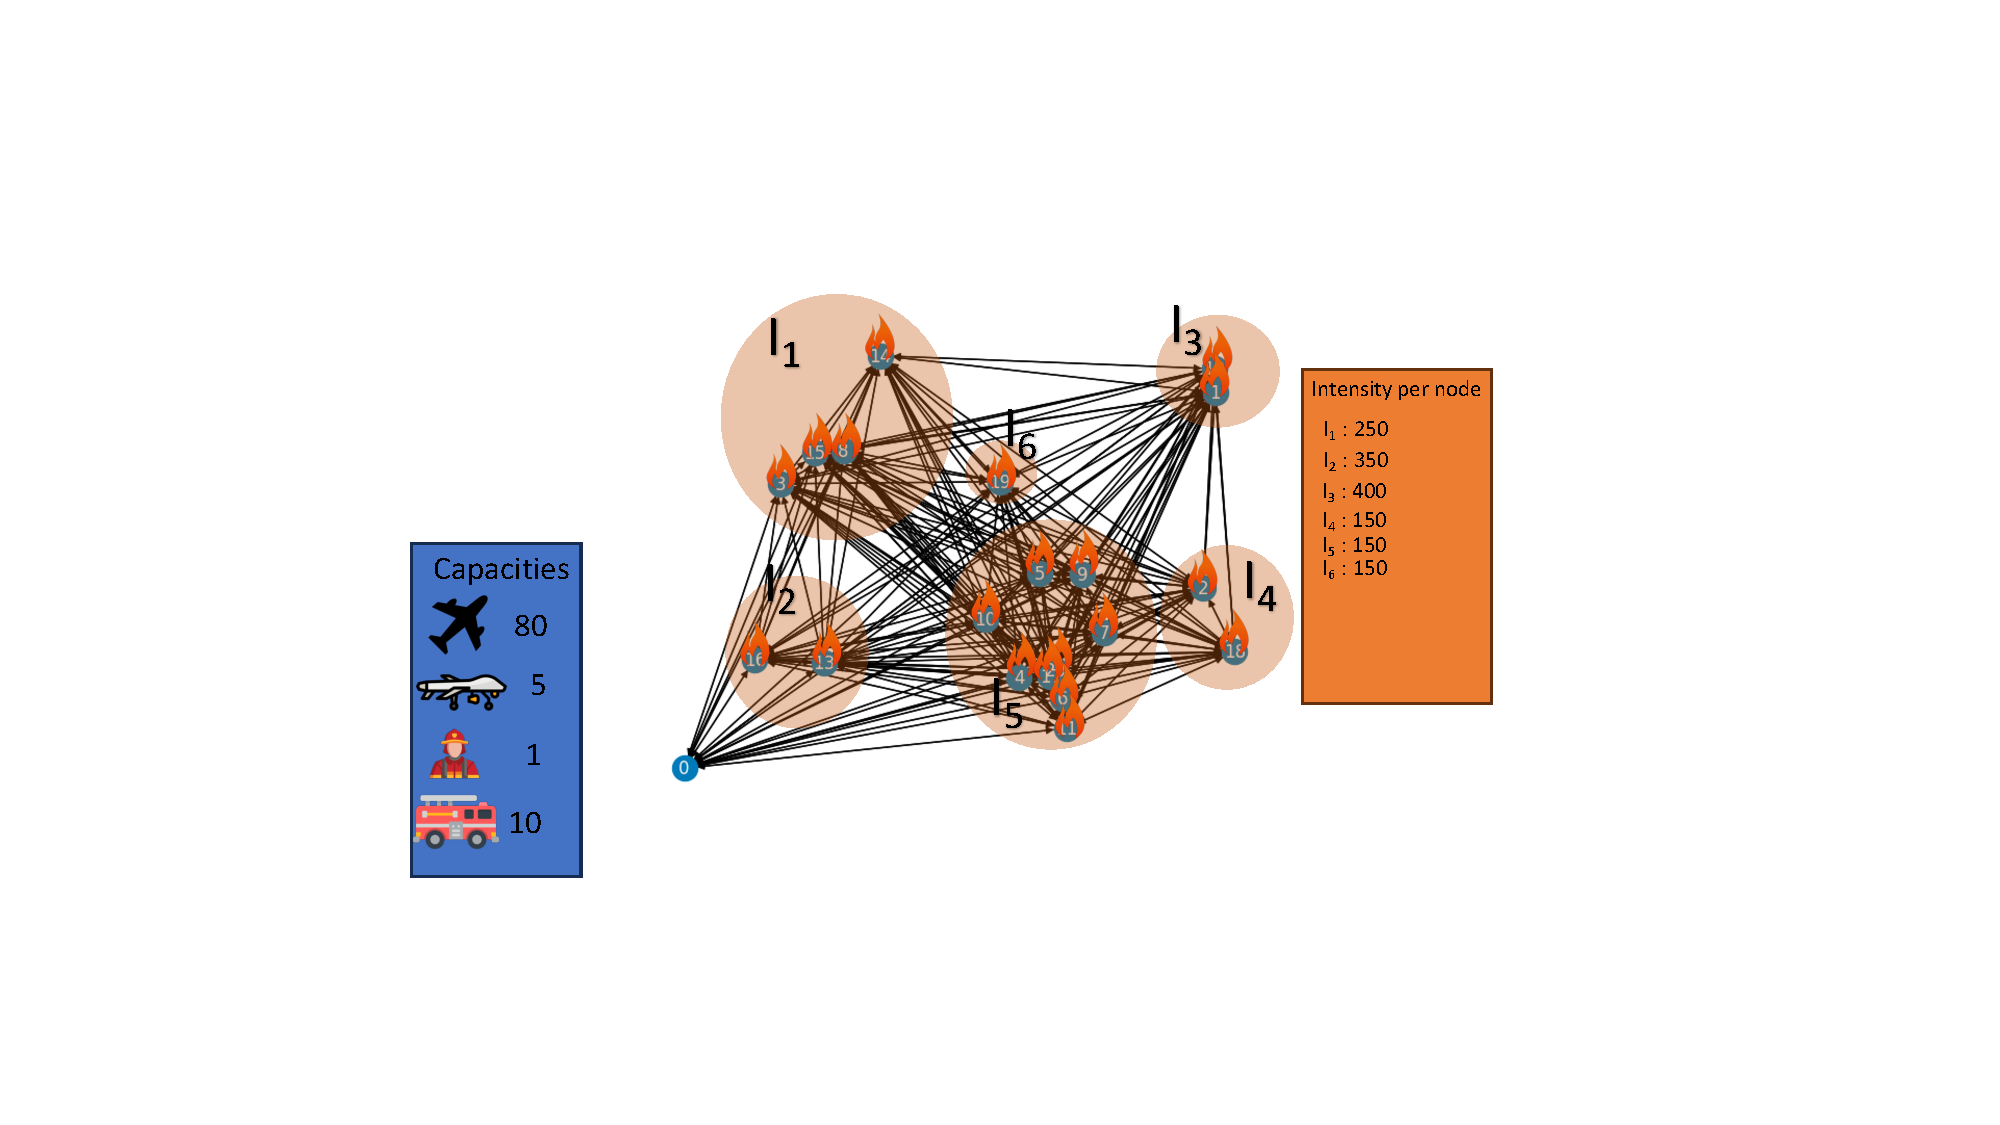
\includegraphics[scale=0.65]{figs/Infograph.pdf}
%\vspace{-10mm}
\caption{Quantified intenside per node is listed on the right while capacities per agent are listed on the left. Wildfire areas are labeled on a basis of fire intensity and agent fire capacity. 
Area shown represents 6 intensity zones and 20 nodes. Node 0 represents the operation based centralized location where all fire equipment will be distributed to the wildfire location. Nodes are extrapolated form the Airnow\copyright official API service and serve as the status of the fire event (Agent). This are recalculated on a temporal basis and re considered for capacity routing purposes.
Internal caracteristics of the agents are considered within the agent-based simulation interacting with the fire event and other agents. Forecasted caracteristics of the fire event are included.}
\label{fig01}
\end{figure}





% \begin{figure}
% \begin{figure}
%   \centering
%   % \texttt{subfigure} with \texttt{[t]}op alignment

%   \medskip

  
%   \begin{subfigure}{0.95\linewidth}
%     \centering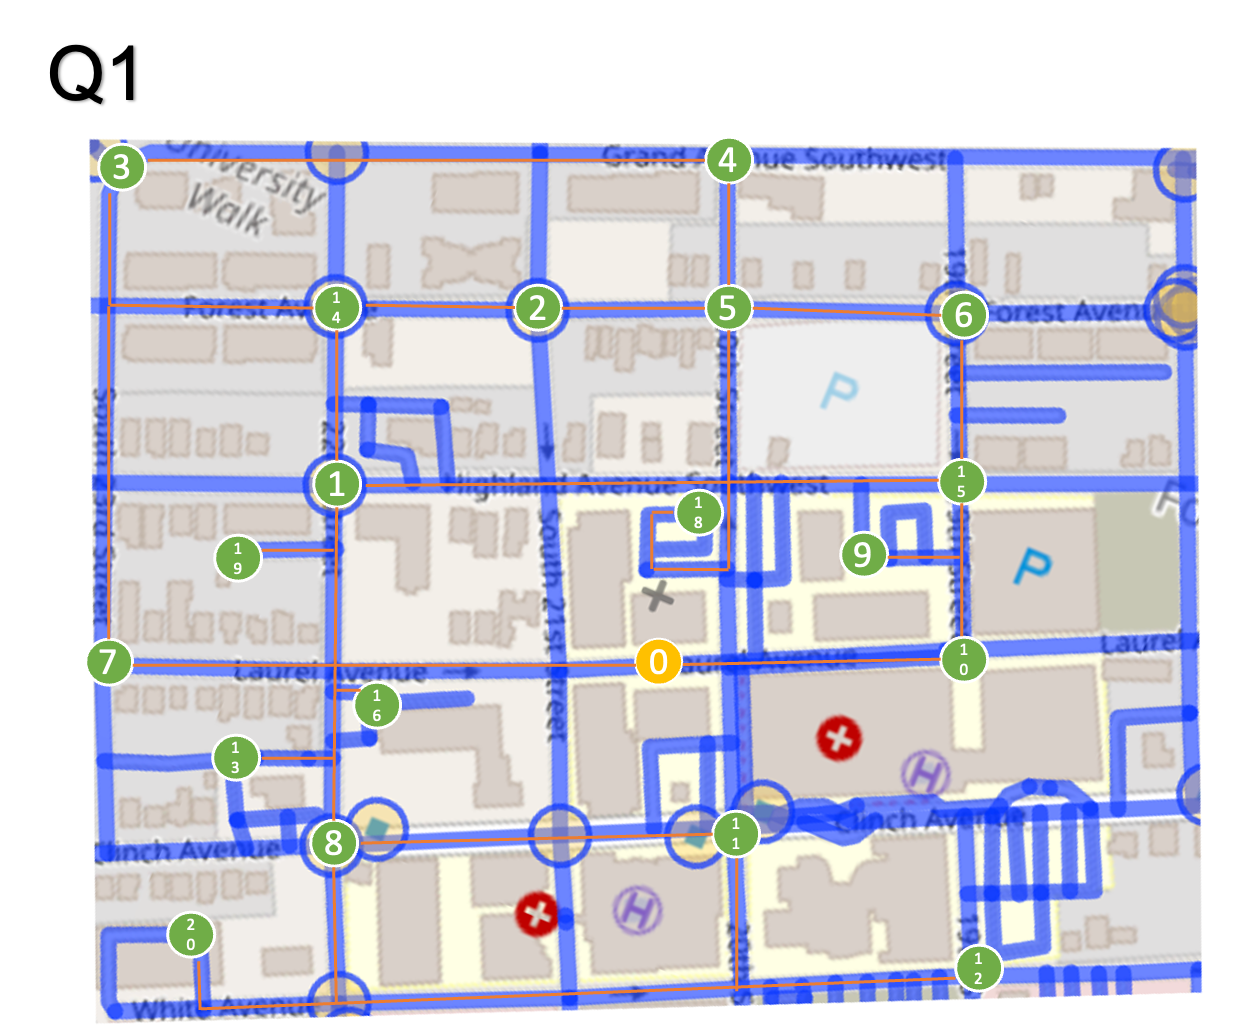
\includegraphics[width=.5\linewidth]{figs/second.png}
%     \caption{First quadrant depicting areas of interest and through the geographic information system software. Illustrated node "0" denotes the initial and ending point of departure of the FVP MAVs.}
%   \end{subfigure}
%   \begin{subfigure}{0.95\linewidth}
%     \centering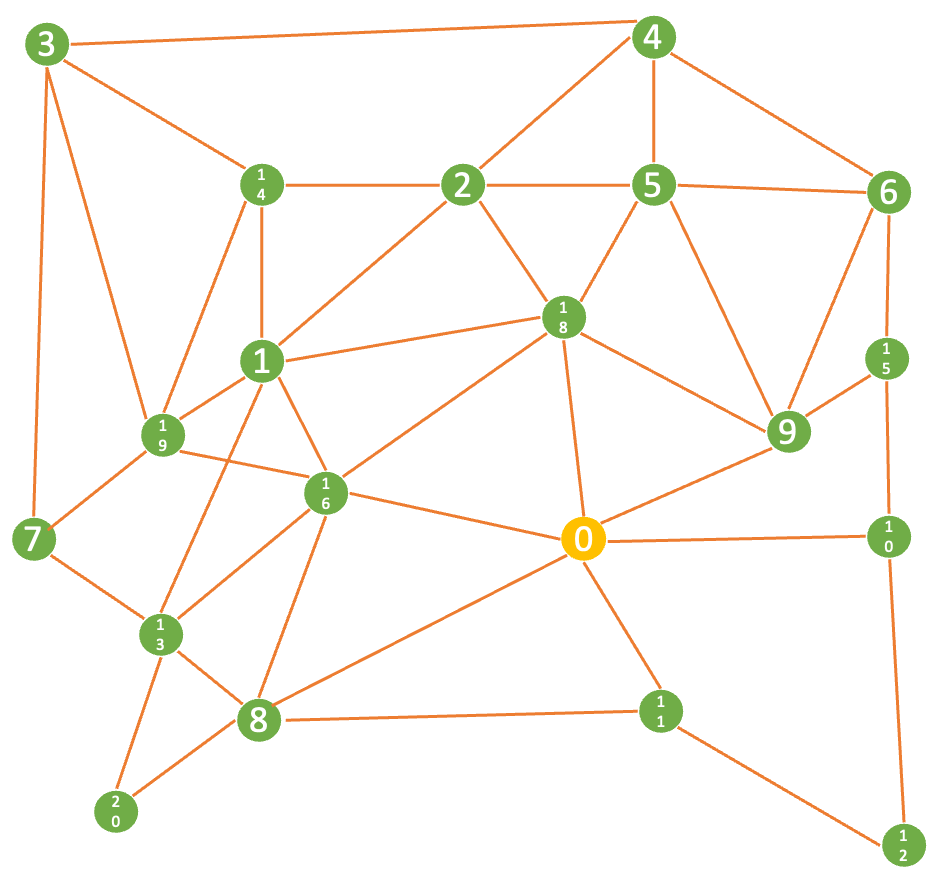
\includegraphics[width=.5\linewidth]{figs/third.png}
%     \caption{Extrapolated POIs to be considered as nodes of for the mTSPGA algorithm}
%   \end{subfigure}
%   \begin{subfigure}{0.95\linewidth}
%     \centering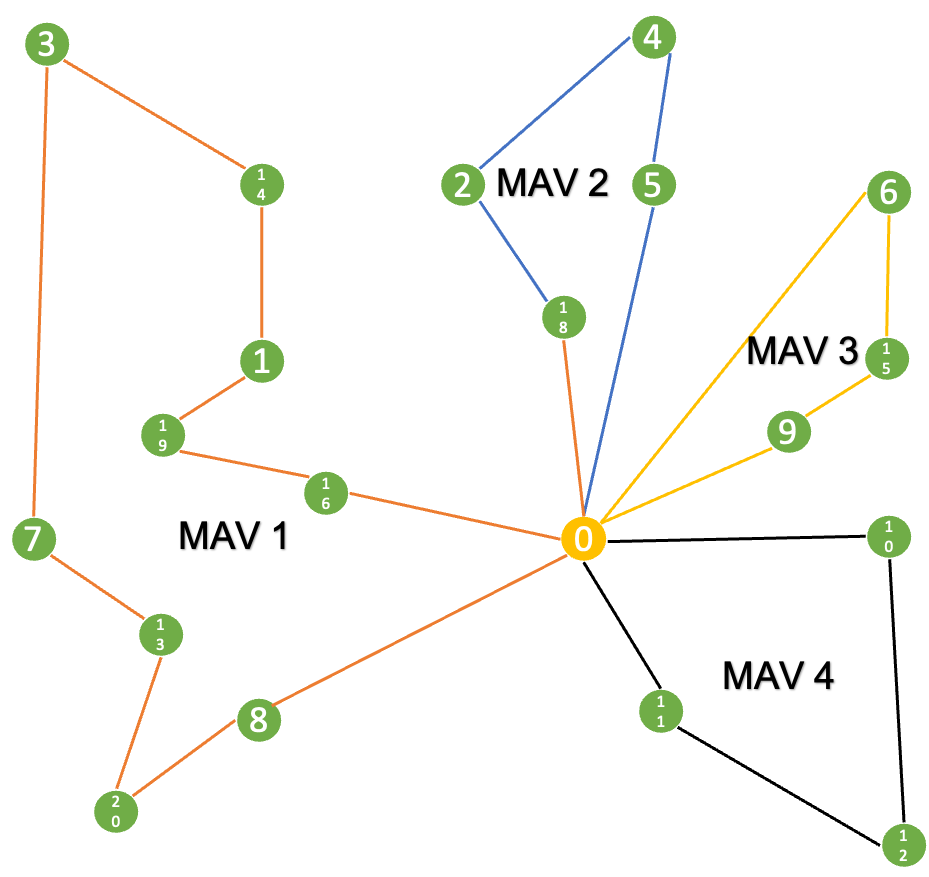
\includegraphics[width=.5\linewidth]{figs/fourth.png}
%     \caption{TSP routing after the application of the genetic algorithms }
%   \end{subfigure}

%   \end{figure}
    % \centering
    % \begin{subfigure}
    % 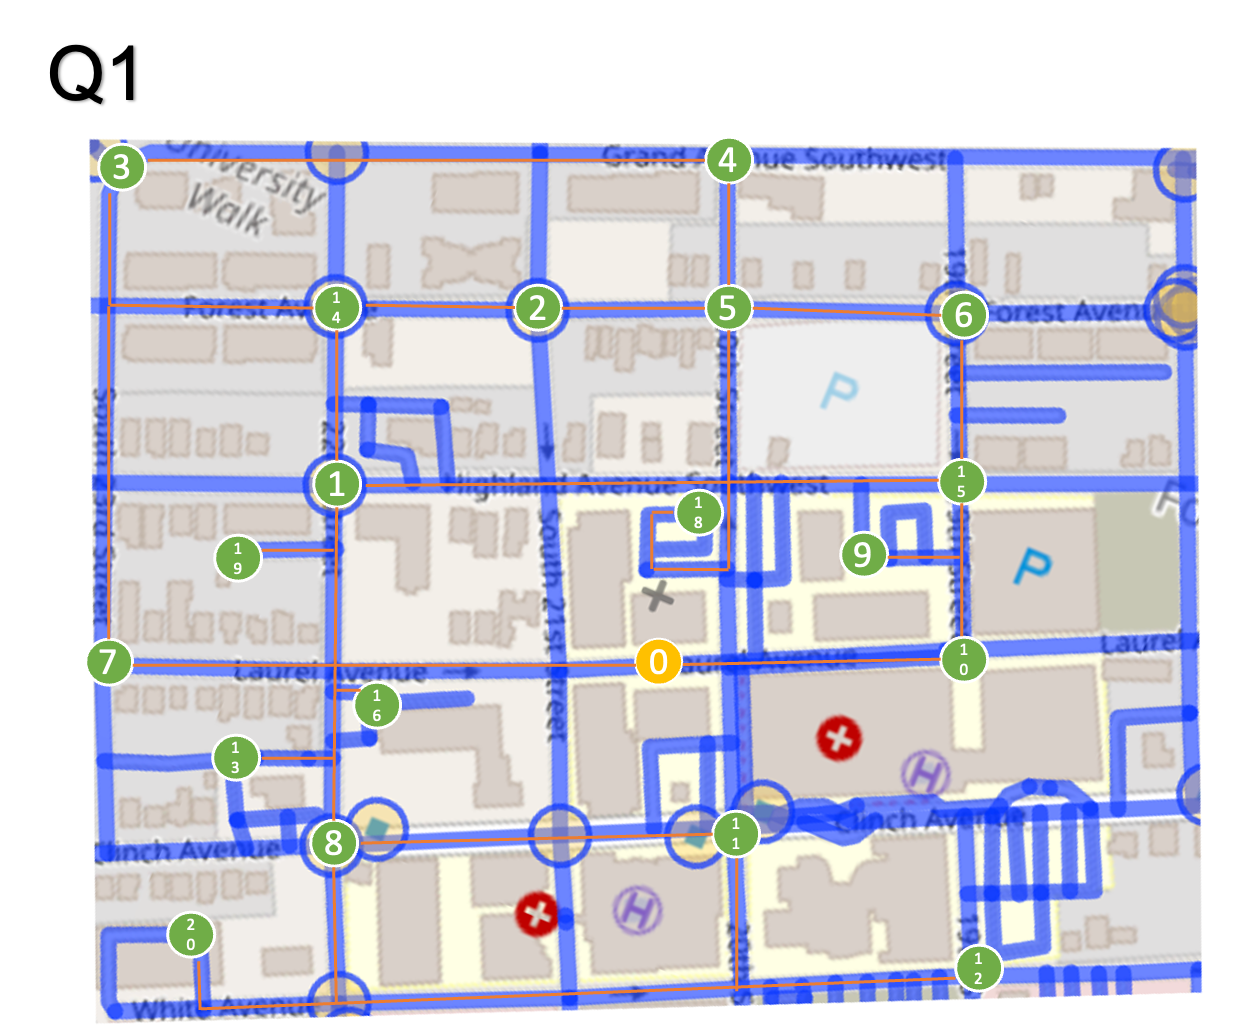
\includegraphics[width=0.60\textwidth]{figs/second.png}
    % \caption{(a) Figure (b) blah (c) blah }
    % \end{subfigure}
    % \begin{subfigure}
    % 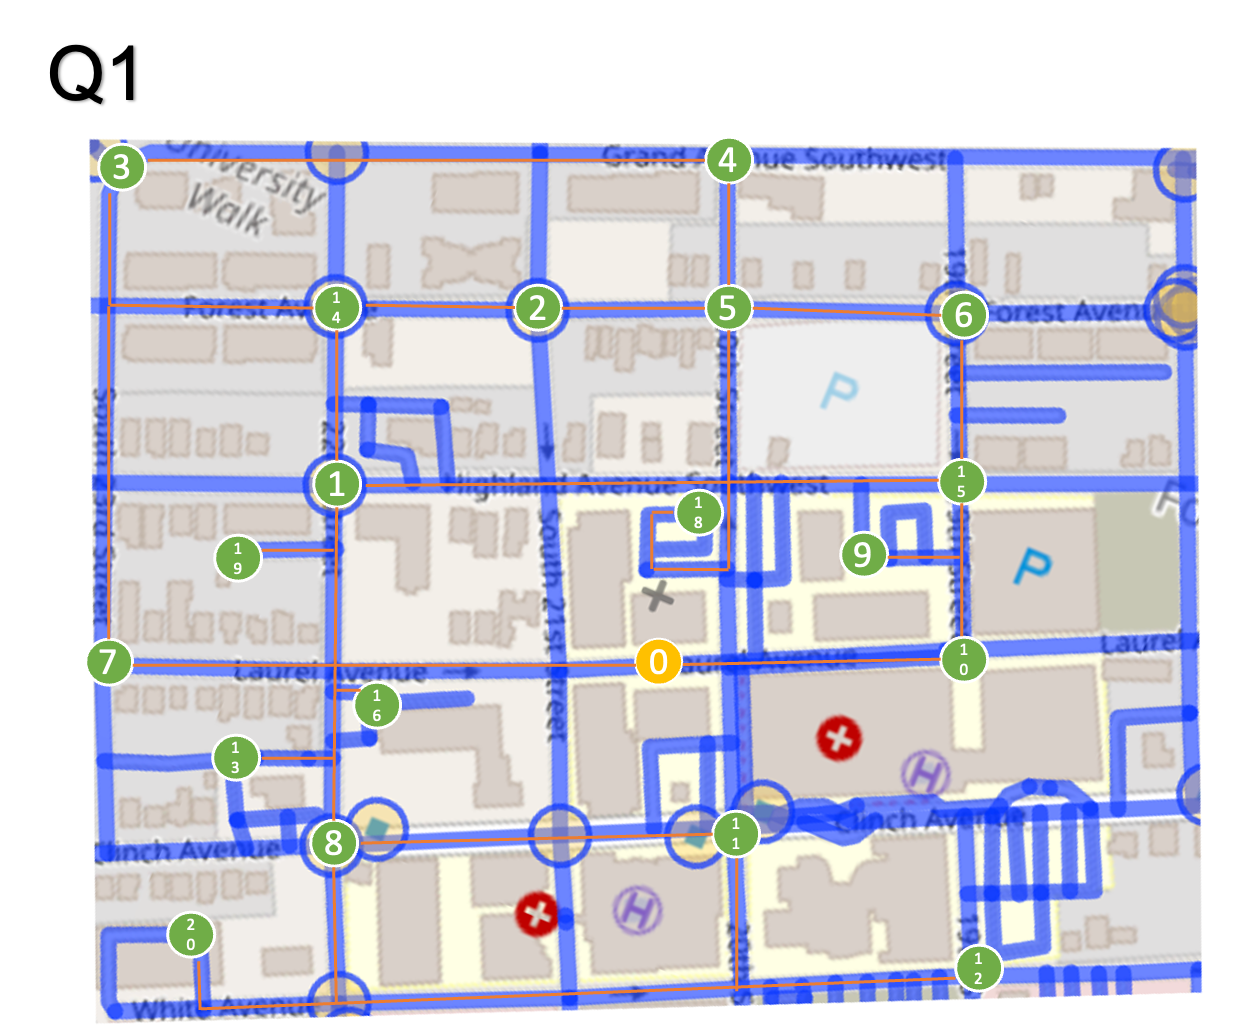
\includegraphics[width=0.60\textwidth]{figs/second.png}
    % \caption{(a) Figure (b) blah (c) blah }s
    % \end{subfigure}
    % % \subfigure{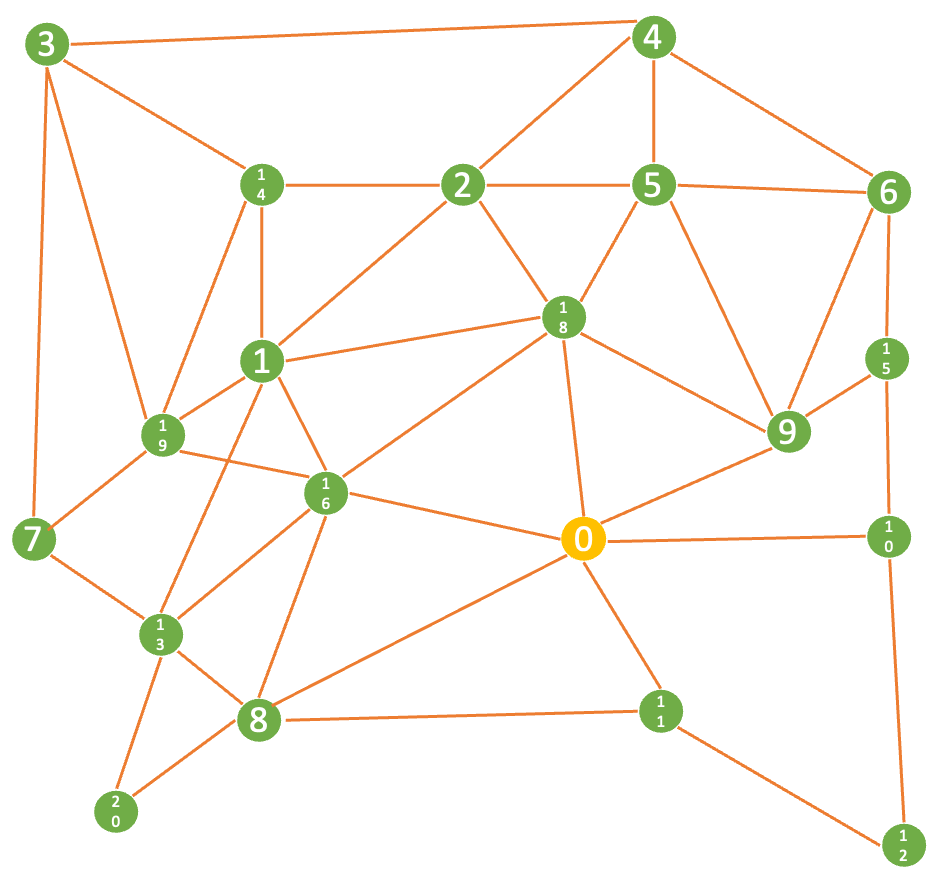
\includegraphics[width=0.48\textwidth]{figs/third.png}} 
    % % \subfigure{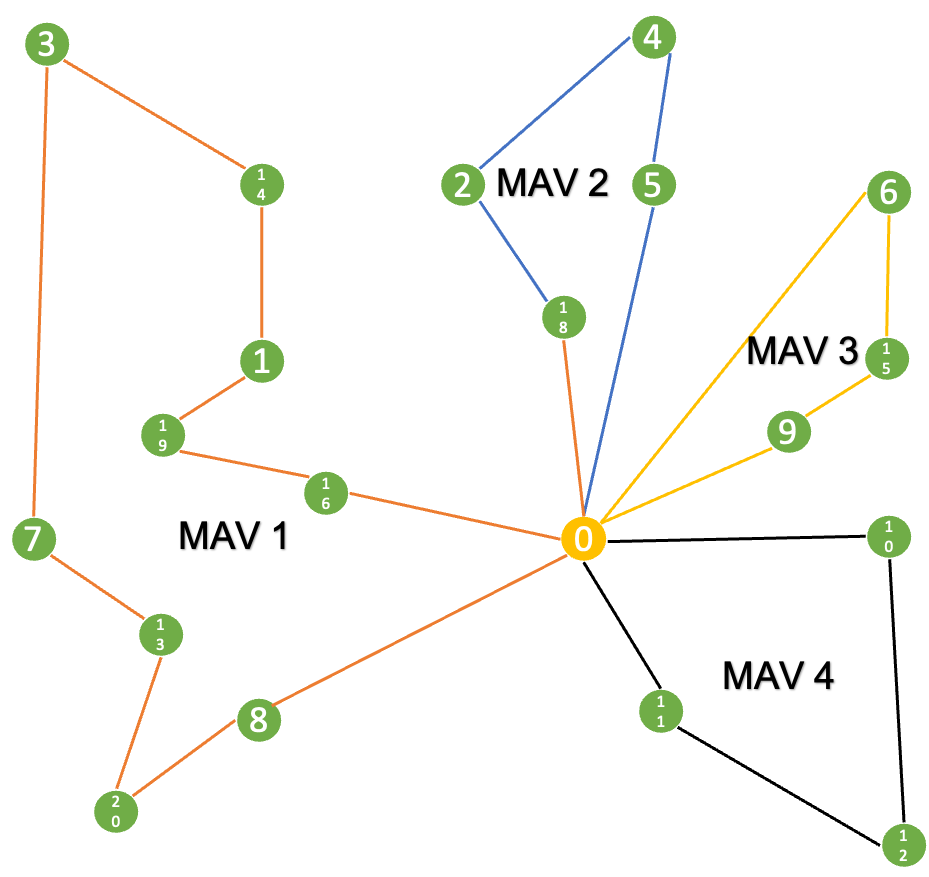
\includegraphics[width=0.48\textwidth]{figs/fourth.png}}
    
    
 
% \end{figure}

% \begin{figure}[!htbp]
% \centering
% 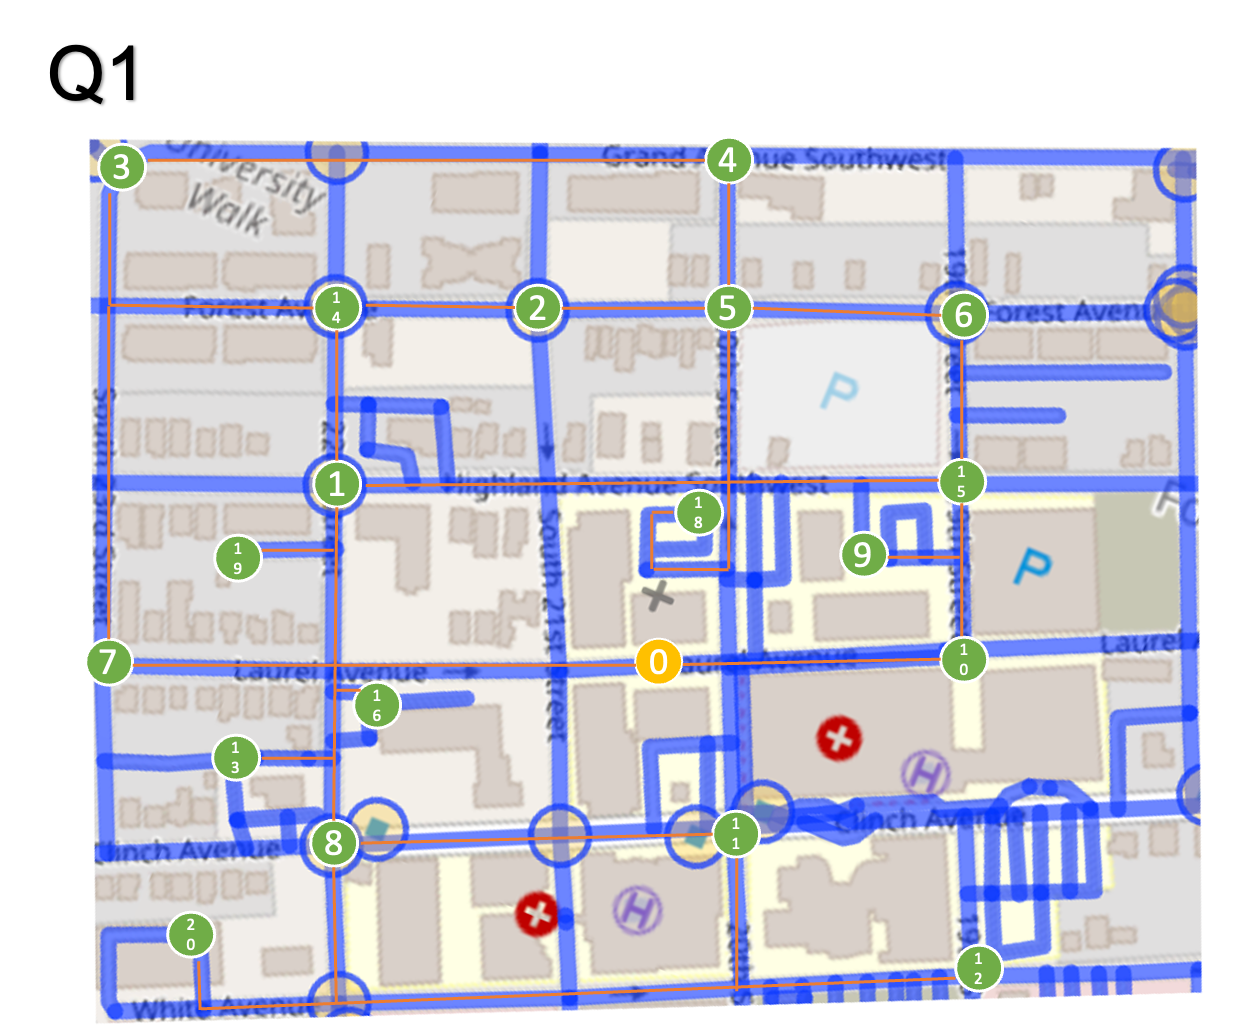
\includegraphics[scale=0.65]{figs/second.png}
% %\vspace{-10mm}
% \caption{Each customer is supplied through a primary and a backup supply route in order to minimize the cost of facility and transportation while considering disruption of the facilities.}
% \label{fig01}
% \end{figure}


% \begin{figure}[!htbp]
% \centering
% 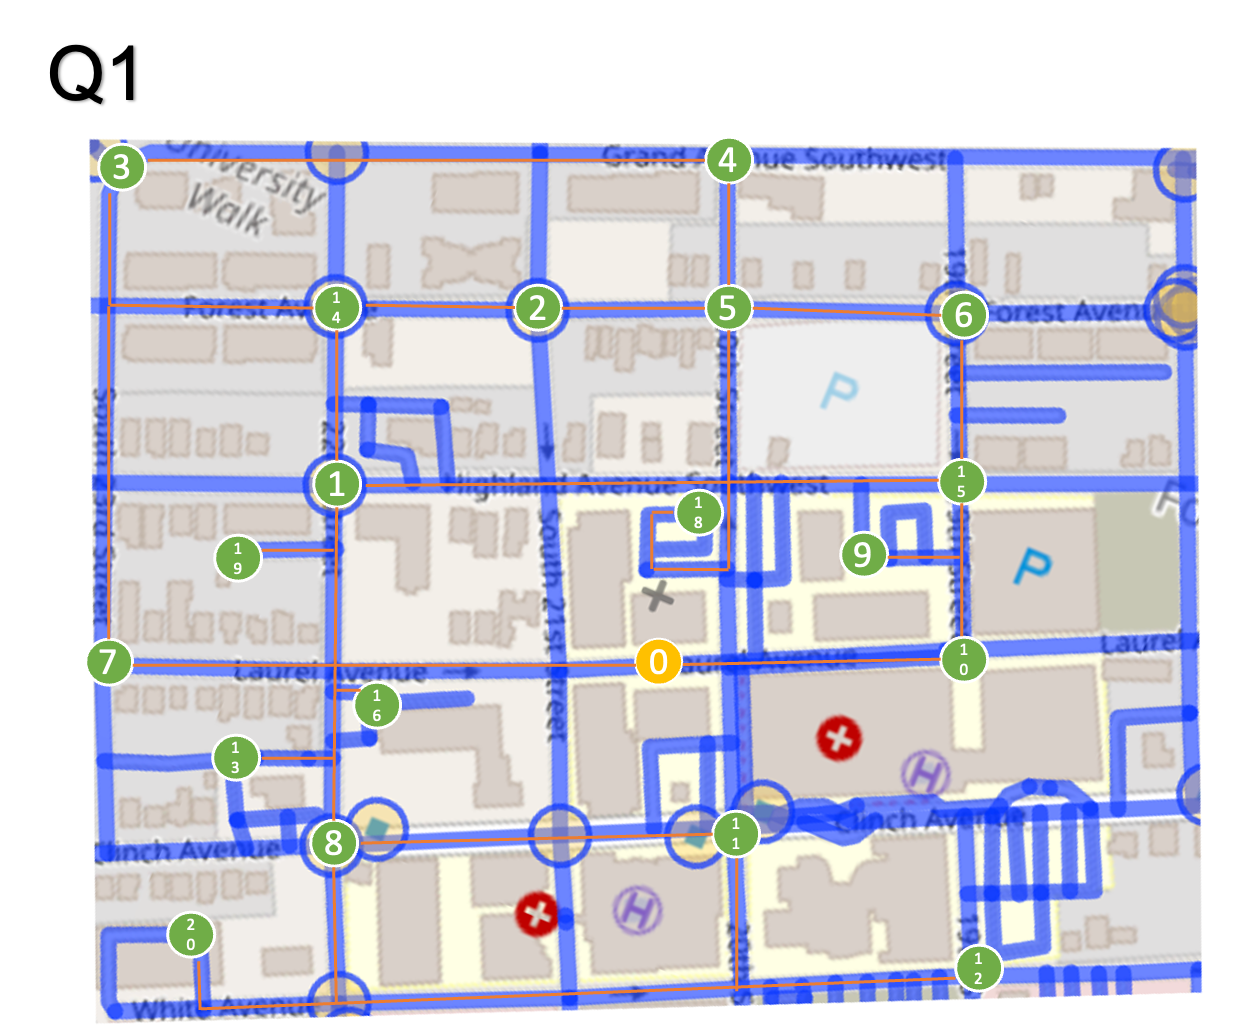
\includegraphics[scale=0.65]{figs/second.png}
% %\vspace{-10mm}
% \caption{Each customer is supplied through a primary and a backup supply route in order to minimize the cost of facility and transportation while considering disruption of the facilities.}
% \label{fig01}
% \end{figure}



% As illustrated in Figure \ref{fig01}, we assign MAVs with a set of AOI locations. That is, AOI is visited and analyzed through the visit of these nodes. Table \ref{Indx} summarizes the notation used in model formulation. \\





%\begin{equation}
% \begin{flalign}
% \label{eq01}
% &\min z = \sum_{i}^{N} \sum_{j}^{N} \sum_{m}^{M}  c_{ijm} x_{ijm} 

% P_{ij\uparrow} + \sum_i \sum_j \sum_{o} \sum_{r} \sum_k \left[c_{rok} x_{ijk} 

% P_{ij\downarrow ro \uparrow} x^\prime_{rok}\right. 
% % &&\\
% % &\left. + \hat{c}_k x^\prime_{rok} P_{ij\downarrow ro \downarrow} x_{ijk} \right]+ \sum_i F_i y_i + \sum_j M_j t_j
% &&\nonumber
% \end{flalign}
%\end{equation}



\section*{Model Formulation}

\textbf{Sets:}
\begin{align*}
& \text{Locations: } \mathcal{L} \\
& \text{Suppliers: } \mathcal{S}
\end{align*}

\textbf{Parameters:}
\begin{align*}
& \text{Cost matrix: } \text{cost\_matrix}_{ij} \quad \forall i, j \in \mathcal{L} \\
& \text{Average demand: } \text{demand\_avg}_i \quad \forall i \in \mathcal{L} \\
& \text{Demand standard deviation: } \text{demand\_std\_dev}_i \quad \forall i \in \mathcal{L} \\
& M \quad \text{(A big-M constant)} \\
& \alpha \quad \text{(Weighting factor for cost)} \\
& \beta \quad \text{(Weighting factor for resource allocation)} \\
& \text{Confidence level low: } \text{confidence\_level\_low} \\
& \text{Confidence level high: } \text{confidence\_level\_high}
\end{align*}

\textbf{Decision Variables:}
\begin{align*}
& x_{ij} \quad \text{(Binary decision variable indicating if a route from location $i$ to $j$ is selected)} \quad \forall i, j \in \mathcal{L} \\
& z_{is} \quad \text{(Binary decision variable indicating if supplier $s$ serves location $i$)} \quad \forall i \in \mathcal{L}, s \in \mathcal{S} \\
& y_i \quad \text{(Continuous decision variable representing the resource allocation at location $i$)} \quad \forall i \in \mathcal{L}
\end{align*}

\textbf{Objective Function:}
\begin{align*}
\text{Minimize:} \quad & \alpha \sum_{i,j \in \mathcal{L}} \text{cost\_matrix}_{ij} \cdot x_{ij} - \beta \sum_{i \in \mathcal{L}} y_i
\end{align*}

\textbf{Constraints:}
\begin{align*}
& \text{Connectivity constraints:} \quad \sum_{j \in \mathcal{L}} x_{ij} = 1 \quad \forall i \in \mathcal{L} \\
& \quad \sum_{i \in \mathcal{L}} x_{ij} = 1 \quad \forall j \in \mathcal{L} \\
& \text{Supplier assignment constraints:} \quad \sum_{s \in \mathcal{S}} z_{is} \leq 1 \quad \forall i \in \mathcal{L} \\
& \text{Resource allocation constraints:} \quad y_i \geq \text{demand\_avg}_i + M \sum_{j \in \mathcal{L}} x_{ij} \quad \forall i \in \mathcal{L} \\
& \text{Stochastic demand constraints:} \quad y_i \geq \text{demand\_avg}_i - \text{demand\_std\_dev}_i \cdot \text{ppf}(1 - \text{confidence\_level\_low}) \quad \forall i \in \mathcal{L} \\
& \quad y_i \leq \text{demand\_avg}_i + \text{demand\_std\_dev}_i \cdot \text{ppf}(1 - \text{confidence\_level\_high}) \quad \forall i \in \mathcal{L} \\
& \text{Confidence level constraints:} \quad \text{cdf}\left(\frac{y_i - \text{demand\_avg}_i}{\text{demand\_std\_dev}_i}\right) \leq \text{confidence\_level\_low} \quad \forall i \in \mathcal{L} \\
& \quad \text{cdf}\left(\frac{\text{demand\_avg}_i - y_i}{\text{demand\_std\_dev}_i}\right) \leq \text{confidence\_level\_high} \quad \forall i \in \mathcal{L}
\end{align*}

% \begin{equation}
% \label{eq01}
% \min z =   \sum_{i,j} lengths_{i,j} *  x_{i,j}
% \end{equation}



% \begin{equation}
% \label{eq02}
% s.t. \sum_{j} x_{i,j} =1, \forall i \in dempoints
% \end{equation}


% \begin{equation}
%   \label{eq02_2}
%   s.t. \sum_{j} x_{i,j} =1, \forall j \in dempoints
%   \end{equation}
  
  


% \begin{equation}
% \label{eq03}
% \sum_{i} x^{(depot,j)} =k  \forall j \in dempoints
% \end{equation}



% \begin{equation}
% \label{eq04}
% u_{i} =q_{i}  \forall  \in dempoints
% \end{equation}


% \begin{equation}
%   \label{eq05}
%   u_{i} =Q  \forall  i  \in dempoints
%   \end{equation}

% \begin{equation}
% \label{eq06}
% q_{depot} = 0 
% \end{equation}


% \begin{equation}
%   \label{eq07}
%    u_{i} - u_{j} + Q * x_{i,j}+ (Q-q_i-q_j) * x_{j,i}<= Q - q_{j} \forall  i,j  \in dempoints  j \not\in depot
%   \end{equation}


% /*
% This has been generated by the overpass-turbo wizard.
% The original search was:
% “Highway”
% */
% [out:json][timeout:25];
% // gather results
% (
%   // query part for: “Highway”
%   node["highway"]({{bbox}});
%   way["highway"]({{bbox}});
%   relation["highway"]({{bbox}});
%        way(area.park)["highway"="footway"];
%      way(area.park)["highway"="pedestrian"];
%      way(area.park)["highway"="path"]; 
 
% );
% // print results
% out body;
% >;
% out skel qt;




% Equation (\ref{eq01})'s goal is to reduce the overall cost of all the agents' travel between the given tasks. Constraints of Equation (\ref{eq02}) ensure that each task is only visited once. While the flow conservation requirements of Equation (\ref{eq03}) mandate that once an agent visits a task, they must also leave it.  Each agent is only utilized once due to the restrictions in Equation (\ref{eq04}), and the subtour elimination constraints in Equation (\ref{eq05}) are ensured by the extra non-negative auxiliary decision variables (sometimes referred to as "node potentials"), with ui corresponding to the ith job. A direct solution strategy may be problematic and unfit for a decentralized implementation because of the NP-hard nature of the mTSPGA. As a result, the strategy in this research is to apply a Genetic Algorithm to heuristicly find the answer. Our model will perform the exploration of nodes or AOI labeled in certain regions $q \in Q$, this covers one of the quadrants in the set $Q$. In order to perform a complete coverage of the area we aim at performing a randomized iterative neighboring area assignation as shown in Figure \ref{Indx}. The highlighted region shows each of the neighboring to be completed in a total area $u \in U$. \\ 



% \begin{algorithm}
% \color{black}
% \begin{algorithmic}
% \STATE Initialize $u$ as an element of $U$
%   % \STATE Initialize $q$ and $q$ as null
% %   \FORALL{$u \in U$}
  
% %   % \STATE Set $q$ as $q[0]$;
%   % \STATE Set $Model$ to problem (\ref{eq01})-(\ref{eq007})
%   % \FORALL{$k \in K$}
%   \STATE Initialize POIs in area $q$ 
  
%   \STATE Separate the universe area into quadrants with a max distance equal to two times the flying distance of the least battery endurance drone. 
%   \FORALL{$q \in Q$}
%     \WHILE{$f(x,y)$ is within conditions }
%   \STATE $f(x,y)$ $<=$ $mTSPGA(POIs,MAVs)$
  
  
  
% \ENDWHILE
%   \RETURN $f(x,y)$ objective function
  
  
%   \ENDFOR
%   % \FORALL{$c^w_{ijrok} \notin Subset$}
%   % \STATE Add $c^w_{ijrok}=0$ to $Model$
%   % \ENDFOR
  
% \end{algorithmic}
% \caption{Pseudo-code for the developed mTSPGA and iterative neighborhood exploration algorithm.\label{Iterative}}

% \end{algorithm}

% The presented Algorithm \ref{Iterative} shows a joint utilization of the mTSPGA algorithm and a neighboring technique to cover certain universe $u$ in the set of universes $U$. $Q$ is an ordered set of adjacent quadrants $q$ so the truck at point "0" is located equidistant from each of the quadrants. Then, 


% \subsection{Genetic Algorithms}
% \label{GeneticAlgo}



% In this model, we assume that suppliers are prone to fail with a known probability distribution. To increase the reliability of the system, each customer is supplied through a pair of primary and backup supply routes, where these two routes cannot be the same for a given customer. That is, at least, one of the facilities in the primary supply route, i.e., depots and satellites, must be different from the facilities in the backup supply route.  

% Equation (\ref{eq01}) shows the objective function of the model which aims to minimize the overall facility setup cost and supply cost through primary and backup suppliers while considering the failure probability of the facilities. Equation (\ref{eq01}) contains the transportation cost of the goods to customers via primary and backup supply routes, while considering their chance of disruption, as well as the setup cost for depots and satellites. Equations (\ref{eq02}) - (\ref{eq03}) account for the assumption that no supply route can play the role of primary and backup supply route for the same customer $k$. Moreover, they dictate the model to chose supply routes only when their respective facilities are installed. As imposed by Equations~(\ref{eq04})~-~(\ref{eq05}), each customer $k$ must be supplied by only one primary and one backup supply route. Equation~(\ref{eq06}) guarantees the  integrity of the binary variables of the model.
% % imply the fact that only through those depots and satellites which are setup, customers can be supplied, for both primary and backup suppliers. Constraints (5) and (6) indicate that each customer must be supplied with only one primary and one backup supplier. Constraint (7) ensures that each supply route can only play the role of primary or backup supplier for a customer while the depot of primary and backup supplier cannot be the same depot due to disruption of depots.
% The cost of supplying customer $k$, $c_{ijk}$, through route $ij$ is calculated by Equation (\ref{Cos}) as
% \begin{equation}
% \label{Cos}
% c_{i,j,k} =  100 d_{k} + 2.5 r_{ijk},
% \end{equation}
% where $d_k$ denotes the order size for customer $k$, and $r_{ijk}$ denotes the length of supply route in~$km$. %times the per $km$ cost to supply customer $k$ through route $i$ and $j$. 
% We set unit cost equal to \$100 and transportation cost equal to \$2.5 per $km$.

% As shown by Equations (\ref{eq02}) - (\ref{eq03}), the same route cannot be assigned to a customer as both primary and backup supply routes, and at least one of the two components of the routes, i.e., depots or satellites, should be different.  
% Hence, three different combinations of depots and satellites can be considered for primary and backup supply routes for a single customer. As shown in Figure \ref{figS}, combination (a) shows two different depots and two different satellites, combination (b) shows a single depot with two distinct satellites, and combination (c) shows two different depots with a single satellite through which a customer can be supplied by primary and backup supply routes.

% \begin{figure}[!htbp]
% \centering
% 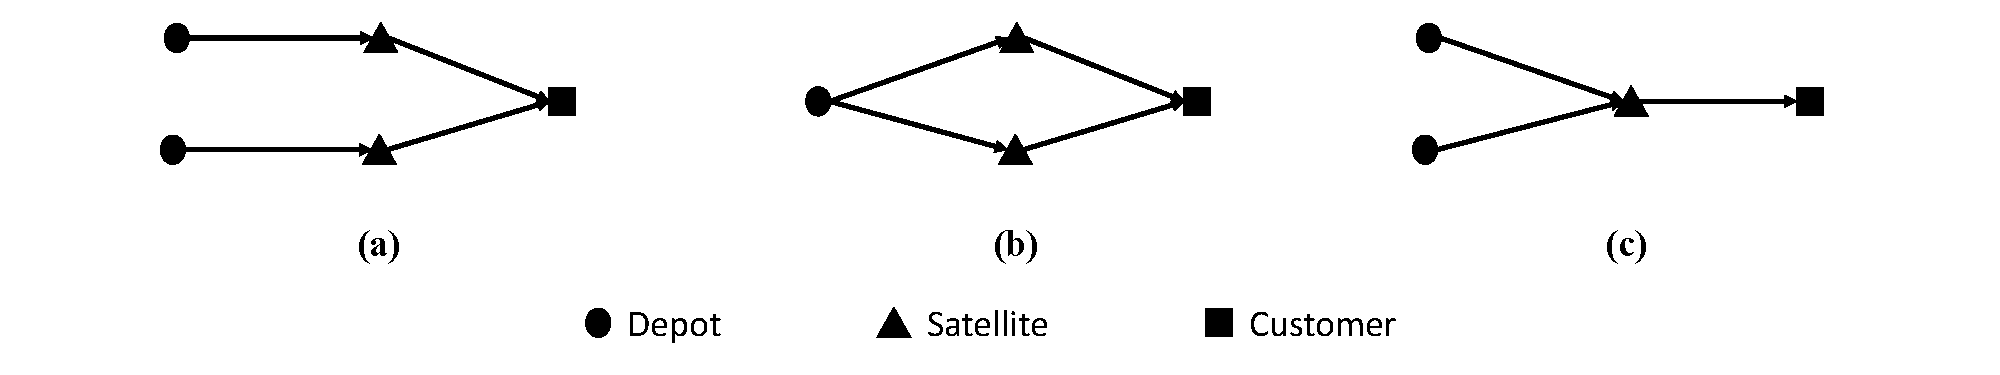
\includegraphics[scale=0.5]{DifferentConnectionTypes.pdf}
% %\vspace{-10mm}
% \caption{Possible combinations of depots and satellites, forming primary and backup supply routes. } 
% \label{figS}
% \end{figure}

% {\color{black}
% The probability that route $i$ and $j$ is up regardless of the type of facility setup is calculated by $p_{ij\uparrow} = (1-p_i)(1-q_j)$, where $p$ is the failure probability for depots and $q$ denotes the failure probability of satellites. 
% The failure probabilities for setup type (a), shown by Figure \ref{figS}, where two depots $i$ and $r$, and two satellites $j$ and $o$ are located is calculated as
% \begin{flalign}
% \label{eq07}
% &p_{ij\downarrow ro\uparrow} = (1-p_r)(1-q_o)(p_i(1-q_j)+q_j(1-p_i)+p_i q_j), &&\\\nonumber
% &p_{ij\downarrow ro\downarrow} = (p_r(1-q_o)+q_o(1-p_r)+p_r q_o)(p_i(1-q_j)+q_j(1-p_i)+p_i q_j),&&\\\nonumber
% \end{flalign}

% \noindent
% the failure probabilities for the setup in which two satellites $j$ and $o$, and one depot $i$ are located, i.e., setup (b) from Figure \ref{figS}, is calculated as
% \begin{flalign}
% \label{eq08}
% &p_{ij\downarrow ro\uparrow} = (1-p_i)q_j(1-q_o),&&\\\nonumber
% &p_{ij\downarrow ro\downarrow} = p_i q_j q_o + p_i (1-q_j)qo + p_i q_j (1-q_o) + p_i (1-q_j)(1-q_o) + (1-p_i) q_j q_o,&&\\\nonumber
% \end{flalign}
% \noindent
% and, for the setup in which two depots $i$ and $r$, and satellite $j$ are setup, i.e., setup (b) from Figure \ref{figS}, the failure probabilities are calculated as
% \begin{flalign}
% \label{eq09}
% &p_{ij\downarrow ro\uparrow} = p_i (1-q_j) (1-p_r),
% &&\\\nonumber
% &p_{ij\downarrow ro\downarrow} =p_i p_r q_j + p_i (1-p_r) q_j + (1-p_i)p_r q_j + p_i p_r (1-q_j),
% &&\\\nonumber
% \end{flalign}
% \noindent
% where $p_{ij\downarrow ro\uparrow} $ and $p_{ij\downarrow ro\downarrow}$ denote the probability of primary route down and backup route up, and primary and backup routes down, respectively.

% % For a special case where all the infrastructures have the same failure probability, $p$, the probabilities for setups (b) and (c) are equal and calculated as\\ 
% % $p_{ij\downarrow ro\uparrow} = p p'^2$, and\\
% % $p_{ij\downarrow ro\downarrow} = p + p^2 p'$,\\
% % where $p' = 1-p$. The failure probabilities for setup (a) are\\
% % $p_{ij\downarrow ro\uparrow} = p'(1-p'^2)$, and\\
% % $p_{ij\downarrow ro\downarrow} = (1-p'^2)^2$,\\
% % which indicate that, in this case, setup (a) is the most robust with a $p_{ij\downarrow ro\uparrow}$ higher than setups (b) and (c), and a lower $p_{ij\downarrow ro\downarrow}$ than other two setups.
% }

% \iffalse
% \begin{table}[!htbp]
% \centering
% \caption{Failure probabilities for under the special case}
% \label{SCSU}
% \footnotesize
% \begin{tabular}{lccc}\toprule
%                                 & \multicolumn{3}{c}{Setup}   \\ \cline{2-4}
% Parameter                       & a          & b &  c  \\ \midrule
% $p_{ij\uparrow} $               & $p'^2$       & $p'^2$ & $p'^2$       \\
% $p_{ij\downarrow ro\uparrow}$   & $p'(1-p'^2)$ & $p p'^2$& $p p'^2$     \\
% $p_{ij\downarrow ro\downarrow}$ & $(1-p'^2)^2$ & $p + p^2 p'$ & $p + p^2 p'$\\ \bottomrule
% \end{tabular}
% \end{table}

% \fi

% %As shown in Table \ref{SCSU}, setups (b) and (c) have the same probabilities, and setup (a) is the most robust with a $p_{ij\downarrow ro\uparrow}$ higher than setups (b) and (c), and a lower $p_{ij\downarrow ro\downarrow}$.
% %\begin{equation}
% %p_{ij\downarrow ro\uparrow} = p'(1-p'^2), \qquad p_{ij\downarrow ro\downarrow} = (1-p'^2)^2 \nonumber
% %\end{equation}

% %


% %p_{ij\downarrow ro\uparrow}$   & $p'(1-p'^2)$     & $p p'^2$                                                \\
% %$p_{ij\downarrow ro\downarrow}$ & $(1-p'^2)^2$  & $p + p^2 p'$ \\

% \subsection{{color{blue}Linearization of the proposed model}}
% \label{METAS}

% In this section, to reduce the solution time of the model, we propose a different mathematical formulation for the developed model in which we {\rev{linearize the previous model and }replace the two primary and backup supply route assignment variables, i.e., $x_{ijk}$ and $x'_{ijk}$, with one variable for each customer $k$. That is, we introduce a new variable, namely, $w_{ijrok}$, which denotes the assigned pair of primary and backup supply routes for each customer $k$. The primary supply route $ij$ and the backup supply route $ro$ are assigned to customer $k$, when $w_{ijrok}$ equals to 1. Note that $i,r \in I$, and $j,o \in J$, where $ij \neq ro$ for all $k$. Through this assumption, we ensure that the same route cannot take the role of main and backup supply routes for the same customer. Moreover, we define the parameter $c^w_{ijrok}$ which denotes the cost of supplying customer $k$ through primary supply route $ij$ and backup supply route $ro$ {\color{black}under disruption probability, i.e.,

% % 
% \begin{equation}
% c^w_{ijrok} = c_{ijk} P_{ij\uparrow} + c_{rok} P_{ij\downarrow ro \uparrow} + \hat{c}_k P_{ij\downarrow ro \downarrow} \qquad \forall i,j,k.
% \end{equation}}



% \begin{flalign}
% \label{eq001}
% &\min W = \sum_i \sum_j \sum_{r \in I} \sum_{o \in J} \sum_k  c^w_{ijrok} w_{ijrok}+ \sum_i F_i y_i + \sum_j M_j t_j&&
% \end{flalign}

% \begin{equation}
% \label{eq002}
% w_{ijrok} \leq y_i \qquad \forall i,j,r,o,k
% \end{equation}
% \begin{equation}
% \label{eq003}
% w_{ijrok}\leq t_j \qquad \forall i,j,r,o,k
% \end{equation}
% \begin{equation}
% \label{eq004}
% w_{ijrok} \leq y_r \qquad \forall i,j,r,o,k
% \end{equation}
% \begin{equation}
% \label{eq005}
% w_{ijrok}\leq t_o \qquad \forall i,j,r,o,k
% \end{equation}


% \begin{equation}
% \label{eq006}
% \sum_{i}\sum_{j}\sum_{r\in I}\sum_{o \in J} w_{ijrok} = 1 \qquad \forall k
% \end{equation}

% \begin{equation}
% \label{eq007}
%  w_{ijrok},y_i,t_j \in \{0,1\} \qquad  \forall i,j,r,o,k.
% \end{equation}\\


% {\color{black}Similar to the objective function of problem (\ref{eq02}) - (\ref{eq07}), the objective function of this model, shown by Equation (\ref{eq001}), 
% aims to minimize the transportation and the facility cost. Note that the objective function also accounts for disruption of the facilities on both levels of depots and satellites.} Equations (\ref{eq002}) to (\ref{eq007}) guarantee that primary and backup supply routes are only through the established depots, while Equation (\ref{eq006}) ensures that only one pair of primary and backup supply routes are allocated to each customer. To reduce the size of the model, Equations (\ref{eq002}) - (\ref{eq004}) can be reformulated as   
% \begin{equation}
% \label{eqNW1}
% \sum_j  \sum_o \sum_k w_{ijrok} \leq M\cdot y_i \qquad \forall i,r,
% \end{equation}

% \begin{equation}
% \label{eqNW2}
% \sum_i \sum_r  \sum_k w_{ijrok} \leq M \cdot t_j \qquad \forall j,o,
% \end{equation}

% \begin{equation}
% \label{eqNW3}
% \sum_{i}\sum_{j}\sum_{r\in I}\sum_{o \in J} w_{ijrok} = 1 \qquad \forall k.
% \end{equation}
% This formulation is the aggregated version of {\color{black}Equations} (\ref{eq002}) - (\ref{eq007}), where $M$ is equal to the number of customers, i.e., $K$, multiplied by 2. The {\color{black}Equations} (\ref{eq002}) - (\ref{eq007}) is theoretically proven to be better than {\color{black}Equations} (\ref{eqNW1}) - (\ref{eqNW3}) as it results to tighter bounds in branch-and-bound algorithm \citep{conforti2014integer}. However, in practice it is observed that the aggregated {\color{black}equations}, i.e., {\color{black}Equations} (\ref{eqNW1}) - (\ref{eqNW3}), perform better as the size of the linear relaxation is much smaller \citep{conforti2014integer}. We exploit this property of the proposed formulation in Section \ref{SCS} while we propose heuristic and meta-heuristic algorithms to speed up the solution process.
% \begin{equation}
% \label{eqNW4}
%  w_{ijrok},y_i,t_j \in \{0,1\} \qquad  \forall i,j,r,o,k.
% \end{equation}\\


%Recall that, as shown by Figure \ref{}, we make the assumption that the same route cannot serve a customer as both primary and backup supply routes. In the first model, Equations (\ref{eq02}) and (\ref{eq03}) guarantee this assumption. In the second mathematical representation of the model, we impose this assumption through the definition of the new introduced variable, i.e., $w_{ijrok}$. That is, we 


% \section{Computational Study}
% \label{SCS}
% The proposed model is an {\rev{INLP}}  with a quadratic objective function. The available commercial solvers, e.g., Gurobi, can solve such INLP models. {\rev{The linear reformulation of the problem helps tackling this issue by reducing the solution time drastically.}} However, for large examples, the model requires a considerable amount of time to be solved. We develop heuristic and meta-heuristic algorithms, namely, {\rev{TS and Route Subset Selector (RSS)}}, in order to improve the time-efficiency of the model while solving for moderate and large examples.

% \subsection{Tabu Search}
% First, we develop a TS for the first model (Equations (\ref{eq01}) - (\ref{eq06})). The developed TS starts by a random selection of a subset of depots and satellites. This is accomplished in the algorithm by randomly assigning zeros and ones to $y_i$ and $t_j$ for all $i \in I$ and $j \in J$, respectively, while maintaining the condition that at least {\color{black} a total of 3 satellites and depots {\rev{(e.g., 2 depots and 1 satellite or 1 depot and 2 satellites)}} have to be installed in order to be able to supply customers through different routes as primary and backup supply routes. Next, for each customer $k$, the algorithm finds a feasible combination of primary and backup routes for which the supply cost for that customer is minimum (considering the disruption probability). Note that the algorithm checks for feasibility of the assigned routes through Equations (\ref{eq03}) and (\ref{eq04}).
% Then, through conducting local search, %either a satellite or a depot is randomly selected, their respective installation variable is changed, and the value for objective function is calculated. This step is repeated until all the possible combinations are covered. The local search is done in the 
% the algorithm randomly switches one $y_i$ or $t_j$ from 0 to 1 and vice versa, and calculates the new objective value. This step is repeated until after a given number of iterations, no improvements are achieved (10 iterations in this study{\rev {, which was chosen empirically}}). The nodes which has been switched is added to the local Tabu list so the algorithm does not switch the same node again while conducting local search.}

% {\color{black}After the local search is completed, the subset of depots and satellites for which the objective value is the smallest is selected. If the objective value for the chosen subset is smaller than that of the best achieved solution, the best achieved solution is replaced with the new subset, the global Tabu list is updated, and local search is conducted on the best solution achieved. However, if the chosen subset does not result in a smaller objective value than that of the best achieved solution, the global Tabu list is checked to ensure that it does not contain the subset. If the subset is in the global Tabu list, the next subset with the smallest objective value is checked until the algorithm finds a subset which is not in the global Tabu list.

% When the new subset is chosen, it is added to the global Tabu list. Then, the new subset is set as the initial solution, and the algorithm goes back to the local search step. The TS algorithm keeps iterating until the stopping criterion is met. In this study, the stopping criterion is when a certain number of iterations are completed and no improvement in the best achieved solution objective value is observed. Note that each time the global Tabu list is updated, if its length surpasses a given value, the oldest entry of the list is removed. Algorithm \ref{TSPS} shows the pseudo-code for the developed TS.}


% \begin{algorithm}
% \color{black}
% \begin{algorithmic}
%   \STATE Set $Tabu\: List$ null;  $improve \gets true$; $Global,Local \gets M$ %$y_i,t_j,x_{ijk},y_{ijk} \gets 0$; Global
%   \STATE Set $Solution$ random 
%   \WHILE{$improve$}
%     \STATE Set $Local\: List$ null; $search \gets true$ 
    
%     %\FOR{$i,j \in Solution$ }
%         \WHILE{$search$}
%         \FORALL{$k \in K$}
%         \STATE %Find $i,j$ and $r,o$ for which the supply cost is minimum; $x_{ijk},x_{rok} \gets 1$
%         %Find main and backup routes for which the supply cost is minimum;
%         $x_{ijk},x_{rok} \gets 1$, for $i,j,r,o \in Solution$, where supply cost is minimum
%         \ENDFOR
%         \STATE Calculate $Local$
%             \IF{$Local \leq Global$}
%                 \STATE $Global \gets Local$
%                 \STATE Update $Tabu\: List$
%             \ENDIF
%             \STATE Conduct Local Search; Update $Local\:List$
            
%             % \IF{no improvements}
%             % \STATE $Local\:Search \gets false$
%             % \ENDIF
%         \ENDWHILE
%     %\ENDFOR
%     \STATE Set $Solution$ equal to subset resulting in $Global$
%     \ENDWHILE
%     \RETURN $Global$
% \end{algorithmic}
% \caption{Pseudo-code for the developed Tabu search.\label{TSPS}}
% \end{algorithm}





% \subsection{Route Subset Selector (RSS)}
% {\color{black}In this section, we develop a heuristic method based on the structure of TUFLPS formulation in order to achieve optimal/near-optimal answers. This method exploits the properties of TUFLP problems, i.e., in order to minimize the cost, it is best to supply the customers with their closest available supplier when capacity is not a constraint. We develop a simple yet effective method based on the mentioned properties by reducing the size of the solution space, i.e., limiting the number of available primary and backup supply routes, for the revised model (\ref{eq001}) - (\ref{eq007}) using constraints (\ref{eqNW1}) - (\ref{eqNW3}).

% We calculate the supply cost for each customer through each pair of primary and backup supply routes considering the disruption probability of facilities, i.e., $c^w_{ijrok}$. Then, a subset of primary and backup supply routes, namely, top n smallest values of $c^w_{ijrok}$ for each customer $k$, are selected, and other primary and backup supply routes for each customer $k$, i.e.,$w_{ijrok}$, are set to~0. This results in a much smaller solution space, especially for large-scale problems.

% The model is solved over the reduced-size solution space via Gurobi. This results in a considerable reduction in solution time while it guarantees a global optima over the selected subset of the chosen routes. The reduction in solution time is more significant for large-scale problems due to the considerable reduction in the size of the solution space over which the problem is solved. Algorithm \ref{RSSPS} shows the pseudo-code for the developed RSS algorithm.}




% \begin{algorithm}
% \color{black}
% \begin{algorithmic}
%   \STATE Set $Subset$ and $c^w$ null;
%   \STATE Set $Model$ to problem (\ref{eq001})-(\ref{eq007})
%   \FORALL{$k \in K$}
%   \STATE Calculate $c^w_{ijrok}$
%   \STATE Update $Subset$ with top $n$ smallest $c^w_{ijrok}$ 
%   \ENDFOR
%   \FORALL{$c^w_{ijrok} \notin Subset$}
%   \STATE Add $c^w_{ijrok}=0$ to $Model$
%   \ENDFOR
%   \RETURN $Model$ objective function
% \end{algorithmic}
% \caption{Pseudo-code for the developed RSS algorithm.\label{RSSPS}}
% \end{algorithm}








% \subsection{Results}
% In this section, we evaluate the reduction in solution time and improvements in the value of the objective function as a result of the implementation of the Tabu search and RSS compared to the commercial solver. That is, we solve the model for 27 different combinations of number of depots, satellites, and customers using the commercial software Gurobi, the developed TS, and RSS and compare the results. The combinations are designed in a way to represent a wide range of different problem sizes for different applications (e.g., small number of candidate sites with a large number of customers (5,5,100), and a large pool for potential candidate sites with only a small number of customers (20,20,10).% The model is solved for the parameter combinations represented in Table \ref{FC2}. 
%  Table \ref{TC} presents the solution time and best solution achieved by the commercial solver and TS, as well as RSS over different number of selected routes.

% \begin{landscape}
% % Please add the following required packages to your document preamble:
% % \usepackage{multirow}
% \begin{table}[!htbp]
% % \color{blue}
% \centering
% \caption{Solution time and objective value difference for the linearized model using commercial solver, TS and RSS.}
% \footnotesize
% \label{TC}
% \resizebox*{1.1\textwidth}{.78\textheight}{
% \begin{tabular}{ccccccccccccccccccccccccc}\toprule
% \multicolumn{3}{c}{Number of Facilities} & IP                                                  & \multicolumn{2}{c}{TS}                                                                                                                      & \multicolumn{2}{c}{Top 10 Routes}            & \multicolumn{2}{c}{Top 100 Routes}            & \multicolumn{2}{c}{Top 500 Routes}           & \multicolumn{2}{c}{Top 1000 Routes}           & \multicolumn{2}{c}{Top 1500 Routes}           \\ \midrule
% Depts    & Sats    & Custs    & \begin{tabular}[c]{@{}c@{}}CPU\\ Time \\ (Seconds)\end{tabular} &
% \begin{tabular}[c]{@{}c@{}}CPU\\ Time\\ (Seconds)\end{tabular} & \begin{tabular}[c]{@{}c@{}}Objective\\ Value\\ Difference\\ (\%)\end{tabular} & 
% \begin{tabular}[c]{@{}c@{}}CPU\\ Time \\ (Seconds)\end{tabular}  & \begin{tabular}[c]{@{}c@{}}Objective\\ Value\\ Difference\\ (\%)\end{tabular} &
% \begin{tabular}[c]{@{}c@{}}CPU\\ Time \\ (Seconds)\end{tabular}  & \begin{tabular}[c]{@{}c@{}}Objective\\ Value\\ Difference\\ (\%)\end{tabular} &
% \begin{tabular}[c]{@{}c@{}}CPU\\ Time \\ (Seconds)\end{tabular}  & \begin{tabular}[c]{@{}c@{}}Objective\\ Value\\ Difference\\ (\%)\end{tabular} &
% \begin{tabular}[c]{@{}c@{}}CPU\\ Time \\ (Seconds)\end{tabular}  & \begin{tabular}[c]{@{}c@{}}Objective\\ Value\\ Difference\\ (\%)\end{tabular} &
% \begin{tabular}[c]{@{}c@{}}CPU\\ Time \\ (Seconds)\end{tabular}  & \begin{tabular}[c]{@{}c@{}}Objective\\ Value\\ Difference\\ (\%)\end{tabular} &
% \\ \midrule
% 5                & 5                    & 10                  & 2.76      & 0.17               & 0.0\%                   & 0.01               & -22.7\%                 & 0.48               & -2.0\%                  & 1.24               & 0.0\%                   & 1.27               & 0.0\%                   & 1.27               & 0.0\%                   \\
% 5                & 5                    & 20                  & 1.40      & 0.59               & 0.0\%                   & 0.02               & 0.0\%                   & 0.11               & 0.0\%                   & 0.45               & 0.0\%                   & 0.72               & 0.0\%                   & 0.59               & 0.0\%                   \\
% 5                & 5                    & 100                 & 27.77     & 3.3                & 0.0\%                   & 0.56               & -0.9\%                  & 3.52               & 0.0\%                   & 34.58              & 0.0\%                   & 45.28              & 0.0\%                   & 48.50              & 0.0\%                   \\
% 5                & 10                   & 10                  & 16.15     & 0.49               & 0.0\%                   & 0.04               & -31.8\%                 & 0.79               & -3.3\%                  & 2.27               & 0.0\%                   & 4.39               & 0.0\%                   & 8.74               & 0.0\%                   \\
% 5                & 10                   & 20                  & 8.46      & 1.7                & 0.0\%                   & 0.07               & 0.0\%                   & 0.15               & 0.0\%                   & 0.51               & 0.0\%                   & 1.07               & 0.0\%                   & 1.76               & 0.0\%                   \\
% 5                & 10                   & 100                 & 190.62    & 7.52               & 0.0\%                   & 0.68               & -4.6\%                  & 1.18               & -0.6\%                  & 22.18              & 0.0\%                   & 47.27              & 0.0\%                   & 83.85              & 0.0\%                   \\
% 5                & 20                   & 10                  & 30.30     & 2.21               & 0.0\%                   & 0.19               & -8.6\%                  & 0.55               & 0.0\%                   & 0.96               & 0.0\%                   & 1.71               & 0.0\%                   & 2.36               & 0.0\%                   \\
% 5                & 20                   & 20                  & 183.28    & 4.82               & 0.0\%                   & 0.56               & -26.4\%                 & 0.90               & -0.2\%                  & 7.04               & 0.0\%                   & 6.48               & 0.0\%                   & 9.32               & 0.0\%                   \\
% 5                & 20                   & 100                 & 341.32    & 32.69              & 0.0\%                   & 2.09               & -5.4\%                  & 5.76               & 0.0\%                   & 22.07              & 0.0\%                   & 29.63              & 0.0\%                   & 31.01              & 0.0\%                   \\
% 10               & 5                    & 10                  & 31.75     & 0.3                & 0.0\%                   & 0.05               & 0.0\%                   & 0.91               & 0.0\%                   & 3.16               & 0.0\%                   & 4.64               & 0.0\%                   & 6.75               & 0.0\%                   \\
% 10               & 5                    & 20                  & 40.36     & 0.79               & 0.0\%                   & 0.10               & -3.9\%                  & 1.90               & -0.9\%                  & 7.13               & 0.0\%                   & 13.06              & 0.0\%                   & 13.02              & 0.0\%                   \\
% 10               & 5                    & 100                 & 20.98     & 5.34               & 0.0\%                   & 0.43               & -1.0\%                  & 1.18               & 0.0\%                   & 13.41              & 0.0\%                   & 26.34              & 0.0\%                   & 51.16              & 0.0\%                   \\
% 10               & 10                   & 10                  & 194.72    & 1.08               & 0.0\%                   & 0.18               & 0.0\%                   & 0.51               & 0.0\%                   & 1.44               & 0.0\%                   & 3.83               & 0.0\%                   & 3.71               & 0.0\%                   \\
% 10               & 10                   & 20                  & 146.55    & 3.4                & 0.0\%                   & 0.45               & -7.5\%                  & 0.62               & 0.0\%                   & 1.21               & 0.0\%                   & 1.89               & 0.0\%                   & 3.71               & 0.0\%                   \\
% 10               & 10                   & 100                 & 240.16    & 25.35              & 0.0\%                   & 2.31               & -12.1\%                 & 2.78               & 0.0\%                   & 15.83              & 0.0\%                   & 34.84              & 0.0\%                   & 56.21              & 0.0\%                   \\
% 10               & 20                   & 10                  & 1,467.86  & 4.92               & 0.0\%                   & 1.09               & 0.0\%                   & 1.56               & 0.0\%                   & 1.72               & 0.0\%                   & 3.28               & 0.0\%                   & 3.48               & 0.0\%                   \\
% 10               & 20                   & 20                  & 1,456.22  & 10.74              & 0.0\%                   & 2.23               & -2.8\%                  & 3.41               & -0.2\%                  & 9.09               & -0.2\%                  & 10.07              & -0.2\%                  & 22.31              & 0.0\%                   \\
% 10               & 20                   & 100                 & 1,185.28  & 80.3               & 0.0\%                   & 13.43              & -5.5\%                  & 16.31              & 0.0\%                   & 31.16              & 0.0\%                   & 33.72              & 0.0\%                   & 59.74              & 0.0\%                   \\
% 20               & 5                    & 10                  & 210.94    & 0.82               & 0.0\%                   & 0.20               & -8.8\%                  & 0.39               & -6.9\%                  & 1.70               & 0.0\%                   & 5.19               & 0.0\%                   & 5.63               & 0.0\%                   \\
% 20               & 5                    & 20                  & 135.31    & 2.03               & 0.0\%                   & 0.41               & -13.4\%                 & 0.62               & 0.0\%                   & 2.61               & 0.0\%                   & 6.54               & 0.0\%                   & 11.79              & 0.0\%                   \\
% 20               & 5                    & 100                 & 10,175.76 & 14.25              & 0.0\%                   & 2.43               & -6.3\%                  & 7.74               & -0.1\%                  & 63.68              & 0.0\%                   & 88.06              & 0.0\%                   & 158.14             & 0.0\%                   \\
% 20               & 10                   & 10                  & 43.12     & 4.76               & 0.0\%                   & 1.12               & 0.0\%                   & 1.64               & 0.0\%                   & 1.85               & 0.0\%                   & 2.92               & 0.0\%                   & 3.78               & 0.0\%                   \\
% 20               & 10                   & 20                  & 190.44    & 12.27              & 0.0\%                   & 2.26               & -1.2\%                  & 3.47               & 0.0\%                   & 5.00               & 0.0\%                   & 5.83               & 0.0\%                   & 7.38               & 0.0\%                   \\
% 20               & 10                   & 100                 & 3,791.42  & 107.51             & 0.0\%                   & 13.73              & -7.0\%                  & 22.25              & 0.0\%                   & 54.27              & 0.0\%                   & 74.60              & 0.0\%                   & 150.53             & 0.0\%                   \\
% 20               & 20                   & 10                  & 199.87    & 21.46              & 0.0\%                   & 7.63               & -17.0\%                 & 8.19               & -1.6\%                  & 8.33               & 0.0\%                   & 8.97               & 0.0\%                   & 11.48              & 0.0\%                   \\
% 20               & 20                   & 20                  & 2,804.34  & 47.09              & 0.0\%                   & 16.43              & -13.0\%                 & 17.57              & -5.2\%                  & 21.83              & -3.6\%                  & 36.46              & -3.2\%                  & 49.48              & 0.0\%                   \\
% 20               & 20                   & 100                 & 12,540.12 & 376.94             & 0.0\%                   & 91.16              & -0.9\%                  & 93.71              & 0.0\%                   & 111.45             & 0.0\%                   & 139.89             & 0.0\%                   & 140.17             & 0.0\%                  
                
% \\ \bottomrule                    
% \end{tabular}}
% \end{table}
% \end{landscape}
% \iffalse
% \begin{landscape}
% % Please add the following required packages to your document preamble:
% % \usepackage{multirow}
% \begin{table}[!htbp]
% \centering
% \caption{Solution time, objective value, gap percentage, and improvements achieved through heuristics.}
% \footnotesize
% \label{TC}
% \resizebox*{1\textwidth}{.6\textheight}{
% \begin{tabular}{ccccccccccccccccccccccccc}\toprule
% \multicolumn{3}{c}{Number of Facilities} & \multicolumn{2}{c}{INLP}                                                  & \multicolumn{2}{c}{TS}                                                                                                                      & \multicolumn{2}{c}{Top 5 Best Routes}             & \multicolumn{2}{c}{Top 10 Best Routes}            & \multicolumn{2}{c}{Top 25 Best Routes}            & \multicolumn{2}{c}{Top 50 Best Routes}            & \multicolumn{2}{c}{Top 100 Best Routes}           & \multicolumn{2}{c}{Top 250 Best Routes}           & \multicolumn{2}{c}{Top 500 Best Routes}           & \multicolumn{2}{c}{Top 1000 Best Routes}          & \multicolumn{2}{c}{Top 2000 Best Routes}          \\ \midrule
% Depts    & Sats    & Custs    & \begin{tabular}[c]{@{}c@{}}CPU\\ Time \\ (Seconds)\end{tabular} &
% Gap (\%) & 
% \begin{tabular}[c]{@{}c@{}}CPU\\ Time\\ (Seconds)\end{tabular} & \begin{tabular}[c]{@{}c@{}}Objective\\ Value\\ Improve\\ (\%)\end{tabular} & 
% \begin{tabular}[c]{@{}c@{}}CPU\\ Time \\ (Seconds)\end{tabular}  & \begin{tabular}[c]{@{}c@{}}Objective\\ Value\\ Improve\\ (\%)\end{tabular} &
% \begin{tabular}[c]{@{}c@{}}CPU\\ Time \\ (Seconds)\end{tabular}  & \begin{tabular}[c]{@{}c@{}}Objective\\ Value\\ Improve\\ (\%)\end{tabular} &
% \begin{tabular}[c]{@{}c@{}}CPU\\ Time \\ (Seconds)\end{tabular}  & \begin{tabular}[c]{@{}c@{}}Objective\\ Value\\ Improve\\ (\%)\end{tabular} &
% \begin{tabular}[c]{@{}c@{}}CPU\\ Time \\ (Seconds)\end{tabular}  & \begin{tabular}[c]{@{}c@{}}Objective\\ Value\\ Improve\\ (\%)\end{tabular} &
% \begin{tabular}[c]{@{}c@{}}CPU\\ Time \\ (Seconds)\end{tabular}  & \begin{tabular}[c]{@{}c@{}}Objective\\ Value\\ Improve\\ (\%)\end{tabular} &
% \begin{tabular}[c]{@{}c@{}}CPU\\ Time \\ (Seconds)\end{tabular}  & \begin{tabular}[c]{@{}c@{}}Objective\\ Value\\ Improve\\ (\%)\end{tabular} &
% \begin{tabular}[c]{@{}c@{}}CPU\\ Time \\ (Seconds)\end{tabular}  & \begin{tabular}[c]{@{}c@{}}Objective\\ Value\\ Improve\\ (\%)\end{tabular} &
% \begin{tabular}[c]{@{}c@{}}CPU\\ Time \\ (Seconds)\end{tabular}  & \begin{tabular}[c]{@{}c@{}}Objective\\ Value\\ Improve\\ (\%)\end{tabular} &
% \begin{tabular}[c]{@{}c@{}}CPU\\ Time \\ (Seconds)\end{tabular}  & \begin{tabular}[c]{@{}c@{}}Objective\\ Value\\ Improve\\ (\%)\end{tabular} &
% \\ \midrule
% 5         & 5             & 10           & 28.11                                                           & 0.00\%   & 0.17                                                           & 0.00                                                                       & 0.02               & -0.28                        & 0.01               & -0.23                        & 0.25               & -0.13                        & 0.49               & -0.08                        & 0.48               & -0.02                        & 0.74               & 0.00                         & 1.24               & 0.00                         & 1.27               & 0.00                         & 1.32               & 0.00                         \\
% 5         & 5             & 20           & 7200                                                            & 8.22\%   & 0.59                                                           & 0.00                                                                       & 0.02               & 0.00                         & 0.02               & 0.00                         & 0.04               & 0.00                         & 0.07               & 0.00                         & 0.11               & 0.00                         & 0.23               & 0.00                         & 0.45               & 0.00                         & 0.72               & 0.00                         & 0.57               & 0.00                         \\
% 5         & 5             & 100          & 7200                                                            & 53.90\%  & 3.30                                                           & 0.02                                                                       & 0.08               & -0.07                        & 0.56               & 0.01                         & 1.20               & 0.02                         & 5.30               & 0.02                         & 3.52               & 0.02                         & 9.20               & 0.02                         & 34.58              & 0.02                         & 45.28              & 0.02                         & 45.49              & 0.02                         \\
% 5         & 10            & 10           & 520.23                                                          & 0.00\%   & 0.49                                                           & 0.00                                                                       & 0.04               & -0.32                        & 0.04               & -0.32                        & 0.07               & -0.32                        & 0.46               & -0.32                        & 0.79               & -0.03                        & 1.73               & -0.03                        & 2.27               & 0.00                         & 4.39               & 0.00                         & 11.12              & 0.00                         \\
% 5         & 10            & 20           & 7200                                                            & 25.77\%  & 1.70                                                           & 0.02                                                                       & 0.08               & 0.00                         & 0.07               & 0.02                         & 0.09               & 0.02                         & 0.12               & 0.02                         & 0.15               & 0.02                         & 0.30               & 0.02                         & 0.51               & 0.02                         & 1.07               & 0.02                         & 2.29               & 0.02                         \\
% 5         & 10            & 100          & 7200                                                            & 83.84\%  & 7.52                                                           & 0.08                                                                       & 0.40               & 0.04                         & 0.68               & 0.04                         & 0.92               & 0.06                         & 2.51               & 0.06                         & 1.18               & 0.08                         & 14.49              & 0.08                         & 22.18              & 0.08                         & 47.27              & 0.08                         & 71.07              & 0.08                         \\
% 5         & 20            & 10           & 7200                                                            & 13.32\%  & 2.21                                                           & 0.00                                                                       & 0.18               & -0.34                        & 0.19               & -0.08                        & 0.22               & 0.00                         & 0.34               & 0.00                         & 0.55               & 0.00                         & 0.91               & 0.00                         & 0.96               & 0.00                         & 1.71               & 0.00                         & 3.03               & 0.00                         \\
% 5         & 20            & 20           & 7200                                                            & 57.24\%  & 4.82                                                           & 0.03                                                                       & 0.42               & -0.35                        & 0.56               & -0.22                        & 0.75               & -0.15                        & 0.86               & -0.01                        & 0.90               & 0.03                         & 3.04               & 0.03                         & 7.04               & 0.03                         & 6.48               & 0.03                         & 12.81              & 0.03                         \\
% 5         & 20            & 100          & 7200                                                            & 78.95\%  & 32.69                                                          & 0.20                                                                       & 2.16               & 0.15                         & 2.09               & 0.16                         & 2.35               & 0.19                         & 2.46               & 0.20                         & 5.76               & 0.20                         & 6.14               & 0.20                         & 22.07              & 0.20                         & 29.63              & 0.20                         & 47.81              & 0.20                         \\
% 10        & 5             & 10           & 181.22                                                          & 0.00\%   & 0.30                                                           & 0.00                                                                       & 0.04               & 0.00                         & 0.05               & 0.00                         & 0.08               & 0.00                         & 0.28               & 0.00                         & 0.91               & 0.00                         & 1.46               & 0.00                         & 3.16               & 0.00                         & 4.64               & 0.00                         & 12.24              & 0.00                         \\
% 10        & 5             & 20           & 7200                                                            & 29.88\%  & 0.79                                                           & 0.01                                                                       & 0.07               & -0.03                        & 0.10               & -0.03                        & 0.45               & 0.00                         & 0.44               & 0.00                         & 1.90               & 0.00                         & 2.60               & 0.01                         & 7.13               & 0.01                         & 13.06              & 0.01                         & 17.10              & 0.01                         \\
% 10        & 5             & 100          & 7200                                                            & 76.30\%  & 5.34                                                           & 0.10                                                                       & 0.40               & 0.09                         & 0.43               & 0.09                         & 0.58               & 0.10                         & 0.81               & 0.10                         & 1.18               & 0.10                         & 4.06               & 0.10                         & 13.41              & 0.10                         & 26.34              & 0.10                         & 14.36              & 0.10                         \\
% 10        & 10            & 10           & 7200                                                            & 32.10\%  & 1.08                                                           & 0.02                                                                       & 0.18               & 0.00                         & 0.18               & 0.02                         & 0.27               & 0.02                         & 0.35               & 0.02                         & 0.51               & 0.02                         & 0.40               & 0.02                         & 1.44               & 0.02                         & 3.83               & 0.02                         & 6.85               & 0.02                         \\
% 10        & 10            & 20           & 7200                                                            & 43.09\%  & 3.40                                                           & 0.01                                                                       & 0.42               & -0.31                        & 0.45               & -0.07                        & 0.38               & 0.01                         & 0.47               & 0.01                         & 0.62               & 0.01                         & 0.75               & 0.01                         & 1.21               & 0.01                         & 1.89               & 0.01                         & 3.69               & 0.01                         \\
% 10        & 10            & 100          & 7200                                                            & 85.06\%  & 25.35                                                          & 0.22                                                                       & 2.26               & 0.11                         & 2.31               & 0.13                         & 2.33               & 0.21                         & 2.47               & 0.22                         & 2.78               & 0.22                         & 7.79               & 0.22                         & 15.83              & 0.22                         & 34.84              & 0.22                         & 52.78              & 0.22                         \\
% 10        & 20            & 10           & 7200                                                            & 58.74\%  & 4.92                                                           & 0.09                                                                       & 1.25               & 0.04                         & 1.09               & 0.09                         & 1.10               & 0.09                         & 1.33               & 0.09                         & 1.56               & 0.09                         & 1.66               & 0.09                         & 1.72               & 0.09                         & 3.28               & 0.09                         & 4.32               & 0.09                         \\
% 10        & 20            & 20           & 7200                                                            & 62.65\%  & 10.74                                                          & 0.17                                                                       & 2.56               & 0.14                         & 2.23               & 0.14                         & 2.89               & 0.14                         & 3.48               & 0.14                         & 3.41               & 0.16                         & 4.35               & 0.16                         & 9.09               & 0.16                         & 10.07              & 0.16                         & 19.75              & 0.17                         \\
% 10        & 20            & 100          & 7200                                                            & 86.20\%  & 80.30                                                          & 0.44                                                                       & 15.32              & 0.40                         & 13.43              & 0.41                         & 13.84              & 0.43                         & 15.81              & 0.44                         & 16.31              & 0.44                         & 21.90              & 0.44                         & 31.16              & 0.44                         & 33.72              & 0.44                         & 92.75              & 0.44                         \\
% 20        & 5             & 10           & 7200                                                            & 25.50\%  & 0.82                                                           & 0.00                                                                       & 0.20               & -0.09                        & 0.20               & -0.09                        & 0.33               & -0.07                        & 0.27               & -0.07                        & 0.39               & -0.07                        & 1.35               & -0.01                        & 1.70               & 0.00                         & 5.19               & 0.00                         & 10.35              & 0.00                         \\
% 20        & 5             & 20           & 7200                                                            & 52.67\%  & 2.03                                                           & 0.06                                                                       & 0.39               & -0.12                        & 0.41               & -0.07                        & 0.56               & 0.06                         & 0.83               & 0.06                         & 0.62               & 0.06                         & 1.71               & 0.06                         & 2.61               & 0.06                         & 6.54               & 0.06                         & 13.29              & 0.06                         \\
% 20        & 5             & 100          & 7200                                                            & 81.84\%  & 14.25                                                          & 0.17                                                                       & 2.24               & 0.08                         & 2.43               & 0.12                         & 3.04               & 0.14                         & 4.86               & 0.16                         & 7.74               & 0.17                         & 9.66               & 0.17                         & 63.68              & 0.17                         & 88.06              & 0.17                         & 196.11             & 0.17                         \\
% 20        & 10            & 10           & 7200                                                            & 59.12\%  & 4.76                                                           & 0.05                                                                       & 1.30               & -0.23                        & 1.12               & 0.05                         & 1.14               & 0.05                         & 1.45               & 0.05                         & 1.64               & 0.05                         & 1.59               & 0.05                         & 1.85               & 0.05                         & 2.92               & 0.05                         & 5.33               & 0.05                         \\
% 20        & 10            & 20           & 7200                                                            & 69.17\%  & 12.27                                                          & 0.25                                                                       & 2.62               & 0.24                         & 2.26               & 0.24                         & 2.28               & 0.25                         & 3.03               & 0.25                         & 3.47               & 0.25                         & 3.42               & 0.25                         & 5.00               & 0.25                         & 5.83               & 0.25                         & 8.65               & 0.25                         \\
% 20        & 10            & 100          & 7200                                                            & 88.14\%  & 107.51                                                         & 0.39                                                                       & 15.35              & 0.31                         & 13.73              & 0.34                         & 15.95              & 0.38                         & 17.99              & 0.39                         & 22.25              & 0.39                         & 25.66              & 0.39                         & 54.27              & 0.39                         & 74.60              & 0.39                         & 216.92             & 0.39                         \\
% 20        & 20            & 10           & 7200                                                            & 69.37\%  & 21.46                                                          & 0.10                                                                       & 8.35               & -0.05                        & 7.63               & -0.05                        & 7.93               & -0.05                        & 8.45               & 0.09                         & 8.19               & 0.09                         & 8.12               & 0.10                         & 8.33               & 0.10                         & 8.97               & 0.10                         & 11.69              & 0.10                         \\
% 20        & 20            & 20           & 7200                                                            & 85.07\%  & 47.09                                                          & 0.43                                                                       & 17.87              & 0.32                         & 16.43              & 0.35                         & 16.62              & 0.37                         & 17.46              & 0.39                         & 17.57              & 0.40                         & 18.92              & 0.40                         & 21.83              & 0.40                         & 36.46              & 0.41                         & 63.83              & 0.43                         \\
% 20        & 20            & 100          & 7200                                                            & 100.00\% & 376.94                                                         & 0.42                                                                       & 90.38              & 0.36                         & 91.16              & 0.41                         & 91.65              & 0.42                         & 92.79              & 0.42                         & 93.71              & 0.42                         & 95.05              & 0.42                         & 111.45             & 0.42                         & 139.89             & 0.42                         & 112.25             & 0.42    \\ \bottomrule                    
% \end{tabular}}
% \end{table}
% \end{landscape}
% \fi

% \iffalse
% \begin{table}[!htbp]
% \centering
% \caption{Solution time, objective value, gap percentage, and improvements achieved through heuristics.}
% \footnotesize
% \label{TC}
% \resizebox*{.95\textwidth}{!}{
% \begin{tabular}{ccccccccccc}\toprule
%                  &                      &                     & \multicolumn{3}{c}{INLP}                         &  & \multicolumn{4}{c}{TS}               \\\cline{4-6} \cline{8-11} 
% \begin{tabular}[c]{@{}c@{}}Number of\\depots\end{tabular}  &\begin{tabular}[c]{@{}c@{}} Number of\\satellites\end{tabular}  &\begin{tabular}[c]{@{}c@{}} Number of\\customers \end{tabular} &\begin{tabular}[c]{@{}c@{}} CPU time\\(seconds)\end{tabular}  & Gap (\%) & \begin{tabular}[c]{@{}c@{}}Objective\\value\end{tabular}  &  &\begin{tabular}[c]{@{}c@{}} CPU time\\(seconds) \end{tabular} &\begin{tabular}[c]{@{}c@{}} Objective\\value \end{tabular} & \begin{tabular}[c]{@{}c@{}} Objective\\value\\improve \end{tabular} & \\ \midrule
% 5  & 5  & 10  & 28.11  & 0\%   & 218,145.07   &  & 0.17   & 218,145.07   & 0.0\%  \\
% 5  & 5  & 20  & 7,200  & 8\%   & 385,574.24   &  & 0.59   & 385,574.24   & 0.0\%  \\
% 5  & 5  & 100 & 7,200  & 54\%  & 1,397,784.64 &  & 3.3    & 1,375,382.63 & 1.6\%  \\
% 5  & 10 & 10  & 520.23 & 0\%   & 191,966.82   &  & 0.49   & 191,966.82   & 0.0\%  \\
% 5  & 10 & 20  & 7,200  & 26\%  & 302,198.61   &  & 1.7    & 294,832.19   & 2.4\%  \\
% 5  & 10 & 100 & 7,200  & 84\%  & 1,810,440.15 &  & 7.52   & 1,661,825.31 & 8.2\%  \\
% 5  & 20 & 10  & 7,200  & 13\%  & 170,285.22   &  & 2.21   & 169,625.10   & 0.4\%  \\
% 5  & 20 & 20  & 7,200  & 57\%  & 359,988.12   &  & 4.82   & 347,723.57   & 3.4\%  \\
% 5  & 20 & 100 & 7,200  & 79\%  & 1,387,172.03 &  & 32.69  & 1,104,640.46 & 20.4\% \\
% 10 & 5  & 10  & 181.22 & 0\%   & 194,929.63   &  & 0.3    & 194,929.63   & 0.0\%  \\
% 10 & 5  & 20  & 7,200  & 30\%  & 354,009.86   &  & 0.79   & 349,975.83   & 1.1\%  \\
% 10 & 5  & 100 & 7,200  & 76\%  & 1,240,562.36 &  & 5.34   & 1,121,211.57 & 9.6\%  \\
% 10 & 10 & 10  & 7,200  & 32\%  & 210,271.02   &  & 1.08   & 205,658.76   & 2.2\%  \\
% 10 & 10 & 20  & 7,200  & 43\%  & 265,412.40   &  & 3.4    & 263,976.93   & 0.5\%  \\
% 10 & 10 & 100 & 7,200  & 85\%  & 1,445,801.49 &  & 25.35  & 1,122,782.97 & 22.3\% \\
% 10 & 20 & 10  & 7,200  & 59\%  & 195,588.20   &  & 4.92   & 178,238.43   & 8.9\%  \\
% 10 & 20 & 20  & 7,200  & 63\%  & 316,993.98   &  & 10.74  & 264,350.59   & 16.6\% \\
% 10 & 20 & 100 & 7,200  & 86\%  & 1,518,558.15 &  & 80.3   & 848,800.32   & 44.1\% \\
% 20 & 5  & 10  & 7,200  & 25\%  & 222,268.79   &  & 0.82   & 222,268.79   & 0.0\%  \\
% 20 & 5  & 20  & 7,200  & 53\%  & 323,729.62   &  & 2.03   & 304,453.13   & 6.0\%  \\
% 20 & 5  & 100 & 7,200  & 82\%  & 1,466,123.16 &  & 14.25  & 1,220,418.67 & 16.8\% \\
% 20 & 10 & 10  & 7,200  & 59\%  & 215,766.47   &  & 4.76   & 204,714.69   & 5.1\%  \\
% 20 & 10 & 20  & 7,200  & 69\%  & 373,973.54   &  & 12.27  & 279,519.90   & 25.3\% \\
% 20 & 10 & 100 & 7,200  & 88\%  & 1,754,932.33 &  & 107.51 & 1,075,017.54 & 38.7\% \\
% 20 & 20 & 10  & 7,200  & 69\%  & 188,635.25   &  & 21.46  & 169,176.79   & 10.3\% \\
% 20 & 20 & 20  & 7,200  & 85\%  & 479,836.97   &  & 47.09  & 275,772.54   & 42.5\% \\
% 20 & 20 & 100 & 7,200  & 100\% & 1,928,975.69 &  & 376.94 & 1,123,596.07 & 41.8\%
%  \\\bottomrule
%  \end{tabular}
% }
% \end{table}
% \fi

% Based on the results shown in Table \ref{TC}, Gurobi commercial solver is able to solve all the cases {\rev{to optimality}} within a time limit of four hours. Note that for cases with a large number of nodes, e.g., (20,5,100), (20,10,100), and (20,20,100), the linearized version of model requires a considerable amount of time to be solved. However, the developed TS and RRS algorithms are able to reach solutions which are as good as the solution achieved by the commercial solver often in a considerably shorter time. Table \ref{TC} shows that the results from RSS heuristic significantly change in the number of selected routes per customer. That is, as the number of selected routes for RSS increases, a larger number of problem settings achieve the optimal objective value as the TS and the linear model. Based on the results shown in Table \ref{TC}, for problem settings with a high level of customers, i.e. 100 customers, a lower number of top routes selected per customer can result in high quality solutions. That is, for the problem settings with (20,20,100), with only 10 routes per customer, we can achieve the optimal value of the objective function, which is less than 0.0001 of the number of routes per customer. Figure~\ref{fig03} shows the trade-off between the number of selected routes, and the improvements in the value of the objective function using RSS method. 
% \begin{figure}[!htbp]
% \centering
% 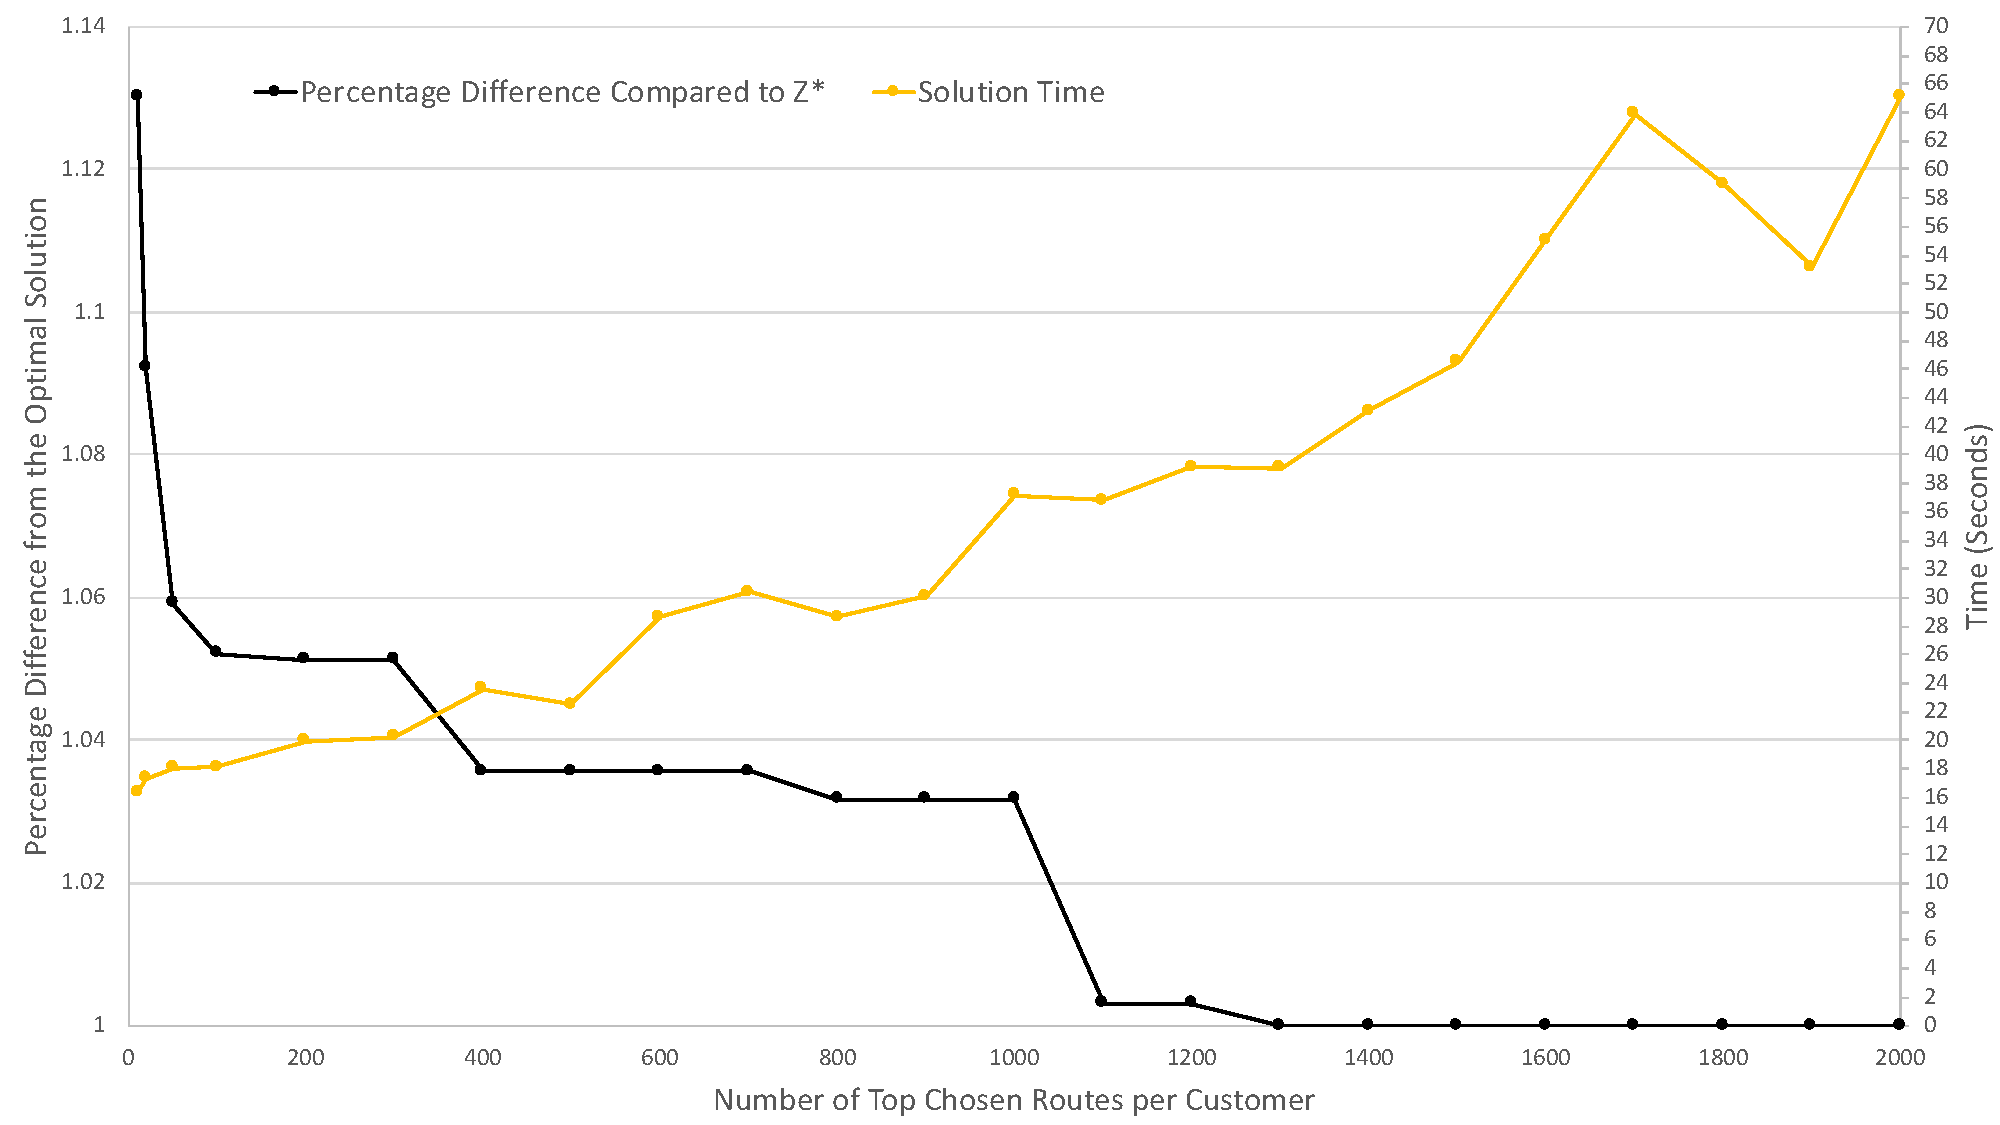
\includegraphics[scale=0.48]{20-20LP.pdf}
% %\vspace{-10mm}
% \caption{The trade-off between improvement in the level of objective function and the solution time based on the number of selected routes per customer for the problem settings with 20 depots, 20 satellites, and 20 customers.}
% \label{fig03}
% \end{figure}

% As Figure \ref{fig03} shows the results for a problem setting of (20,20,20), with only 1,300 routes per customer, i.e., less than 1\% of routes per customer, RSS method achieves the optimal solution, i.e., Z$^*$, in less than 40 seconds. The results show the noticeable effects of reduction in the solution space due to implementation of RSS method.


% Figure \ref{fig04} shows the comparison between the solution time for the developed TS and RSS. Note that the solution times shown for each problem setting for RSS are for the smallest number of top $n$ routes with which RSS reached the best answer. As the figure shows, the solution time for RSS is considerably lower for problem settings with large numbers of main and backup supply routes, i.e., large number of depots, satellites, and customers. For example, for problem settings with 100 customers, the reduction in solution time for RSS compared to the developed TS ranges between [96\%-99\%]. For the problem settings with small numbers of primary and backup supply routes, i.e., small number of depots, satellites, and customers, while the solution time for the developed TS dominated by the solution time for RSS method, in general these settings have short solution times for both methods.


% \begin{figure}[!htbp]
% \centering
% 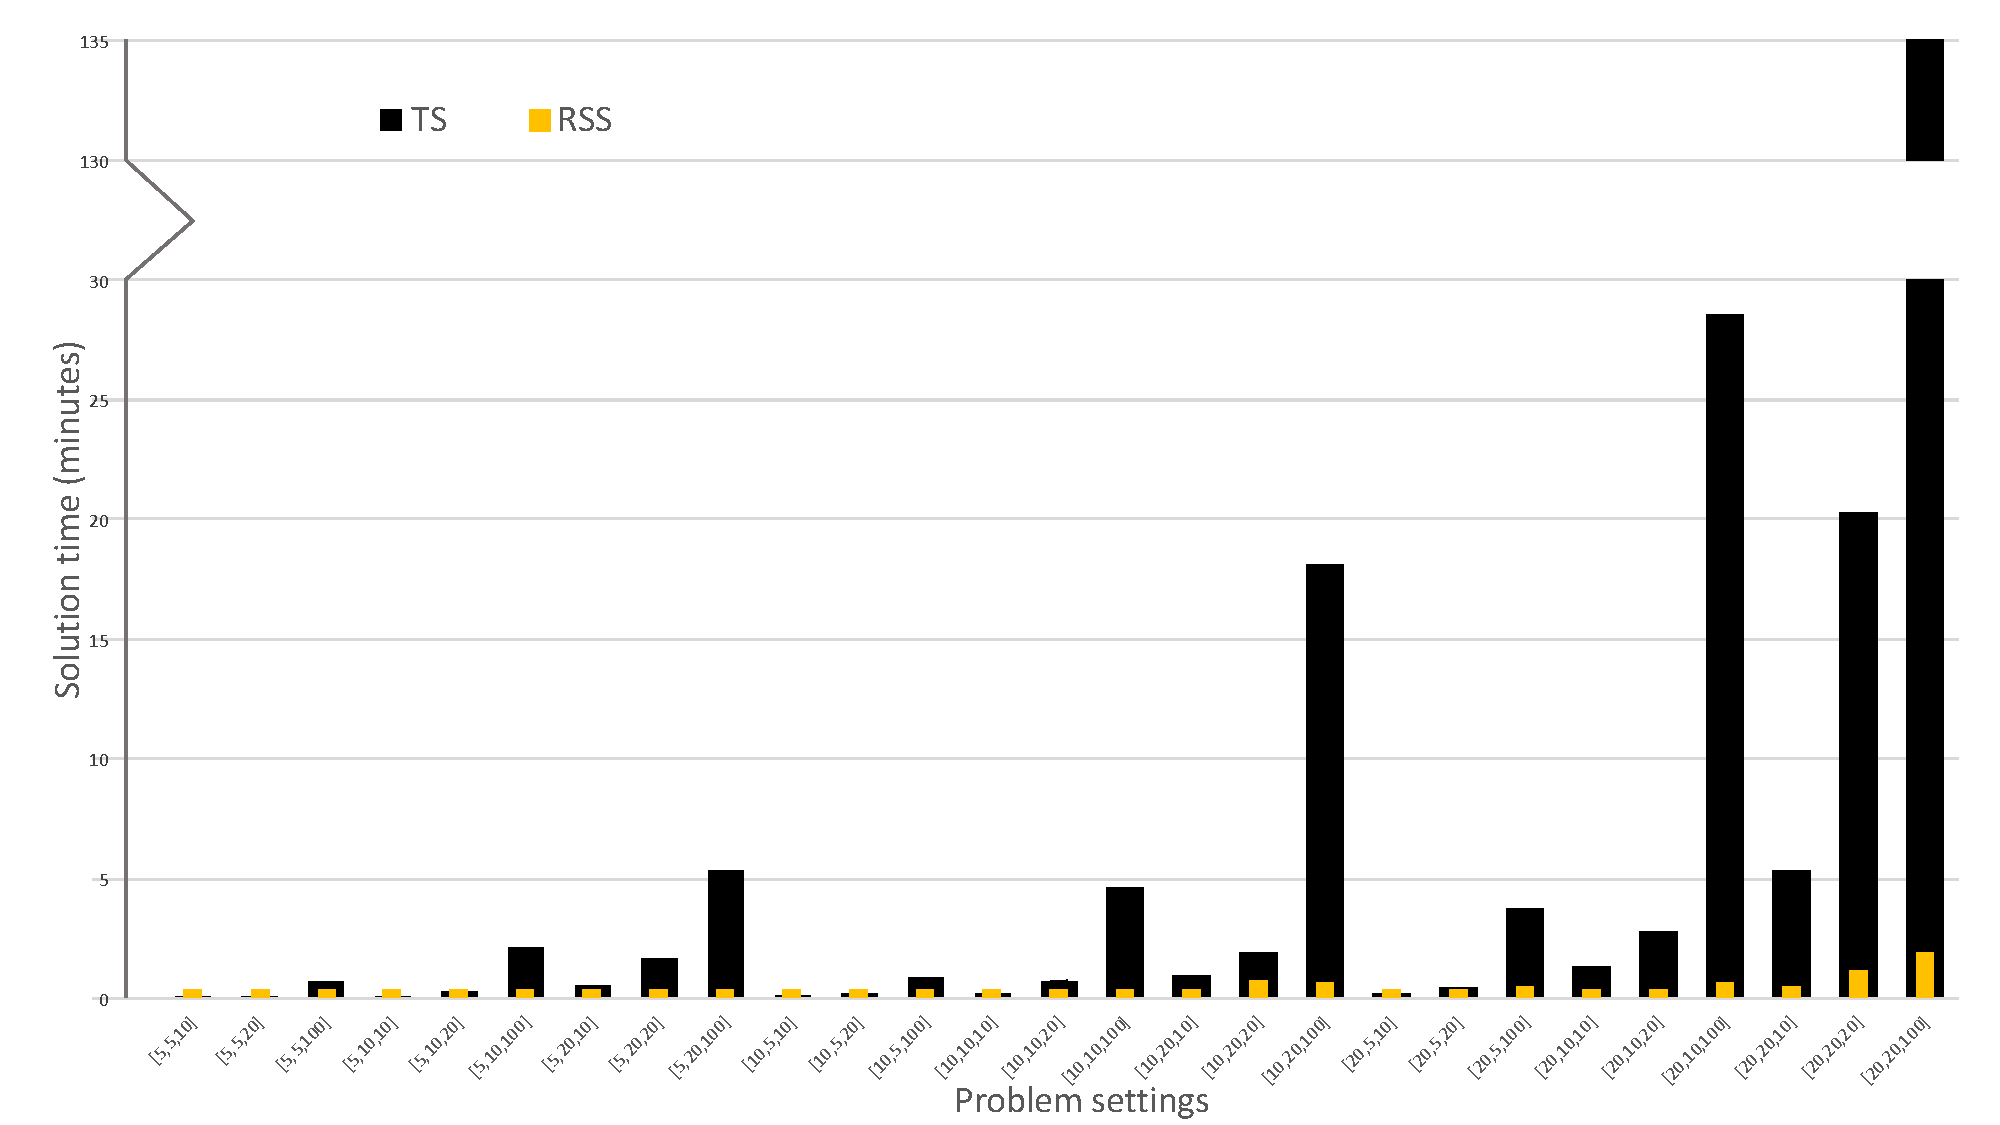
\includegraphics[scale=0.48]{TS-MHComp.pdf}
% %\vspace{-10mm}
% \caption{Comparison of the solution time for TS and the best achieved solution for RSS over different problem settings.}
% \label{fig04}
% \end{figure}



% % \noindent
% % \subsection{Sensitivity and Robustness Analyses}
% % \label{SA} 
% % In this section, we aim to study the effect of failure probabilities on the outcomes of the model. We design a hypothetical small example of 3 depots, 3 satellites, and 5 customers, in order to observe the behavior of the model by changes in the failure probability of the model infrastructures. The parameter settings for the problem are shown in Table \ref{FC} and Table \ref{Probs}.

% % \begin{table}
% % \centering
% % \caption{Fixed cost, and failure probability for each depot $i$ and satellite $j$.}
% % \footnotesize
% % \label{FC}
% % \begin{tabular}{lccc}\toprule
% %                                      & \multicolumn{3}{c}{Index} \\ \cline{2-4}
% % Parameter                            & 1       & 2      & 3      \\\midrule
% % setup cost for depot $i$, $F_i$     & 84,700  & 77,300 & 61,400 \\
% % setup cost for satellite $j$, $M_j$ & 16,800  & 19,600 & 17,300\\ 
% % %Probability that depot $i$ fail, $q_i$&	0.23&0.35	&0.12	\\ 
% % %Probability that satellite $j$ fail, $p_j$&	0.2	& 0.15	& 0.12	\\
% % \bottomrule
% % \end{tabular}
% % \end{table}


% % \begin{table}
% % \centering
% % \caption{Distance to be traveled through each depot and satellite pair to each customer and demand for each customer.}
% % \footnotesize
% % \label{Probs}
% % \begin{tabular}{cccccccc}\toprule
% % \multicolumn{2}{c}{Distance}&  & \multicolumn{5}{c}{Customer} \\\cline{1-2}\cline{4-8}
% % Depot& Satellite& & 1    & 2   & 3   & 4   & 5   \\\midrule
% % 1     & 1         && 377  & 646 & 242 & 454 & 996 \\
% % 1     & 2         && 590  & 341 & 124 & 386 & 903 \\
% % 1     & 3        & & 605  & 121 & 223 & 999 & 263 \\
% % 2     & 1        & & 817  & 916 & 811 & 983 & 245 \\
% % 2     & 2        & & 744  & 577 & 933 & 849 & 895 \\
% % 2     & 3        & & 515  & 929 & 538 & 392 & 249 \\
% % 3     & 1         && 341  & 378 & 736 & 566 & 629 \\
% % 3     & 2        & & 287  & 941 & 167 & 754 & 272 \\
% % 3     & 3        && 152  & 346 & 888 & 570 & 320\\\midrule
% % \multicolumn{2}{c}{Demand}&&191&20&26&169&150\\\bottomrule
% % \end{tabular}
% % \end{table}

% \section{Conclusion and Remarks}
% \label{Con}
% {\rev{In this paper, we studied a two level facility location problem with single assignment under disruption probability in order to find the optimal locations for two different layers of facilities as well as the optimal primary and back up route assignment for customers. We assume that facilities in different levels, i.e., depots and satellites, are independently prone to disruptions. We proposed two formulations for the problem and developed a TS algorithm and RSS, a problem specific heuristic. We then compared their performance with the answers from solving the linear formulation using Gurobi, and with one another over 27 different problem settings. The results show that the proposed TS and RSS outperform Gurobi. That is, Gurobi is able to solve all the problem instances in less than four hours. However, TS and RSS can reduce the solution time considerably. The results also show that while the differences between the solution times for TS and RSS are negligible over small problem settings, RSS outperforms over TS on large problem settings, i.e., with 100 customers. We conducted sensitivity analysis on number of routes used in RSS. The solution and the quality of the achieved answers via RSS significantly relies on the number of routes selected per customer. While a smaller number of routes per customers selected can reduce the solution time by a large margin, it can also drastically reduce the quality of the achieved solutions. As a result, while RSS can outperform the basic TS developed in this study over the large case studies, it requires a higher level of hyper-parameter tuning.

% The problem under study, TUFLP, can find its applications in a variety of scenarios wherein the locations of certain facilities could have substantial impacts on the system. For instance, under the context of supply chain network design and supply disruptions, one may need to determine the locations of distribution centers (DCs, i.e., depots in the proposed model) and local distribution centers (LDCs, i.e., satellites), how to assign retailers and customers to LDCs, and under disruptions, which backup DCs and LDCs should be used. Such decisions are critical to the overall supply chain performance and are closely related to supply chain resilience. The developed mathematical formulation and solution methods can be directly applied to such problems.     

% Future studies can consider the disruption probability in models with a higher number of levels. Also, it is of interest to study the problem under different disruption scenarios for different facilities. For example, the disruption probability at each facility can be correlated to or independent of each other.}}


% \section{Acknowledgments} 
% {\rev{The authors thank the editor and reviewers for their constructive and helpful comments. The work was support in part by the National Science Foundation Grant CMMI-xxxxxxx (\textit{hidden for peer review}).}}


% \subsection{Linearizatin Process}
% The proposed model is a NLIP with quadratic objective function. The available commercial solvers such as Gurobi can solve such INLP models. Nevertheless, to reduce the computational efforts, we convert the quadratic objective function into a linear one by introducing a new binary variable, namely $n_{i,j,r,o,k}$, and its corresponding set of constraints. That is, since the non-linearity of the objective function is due to a multiplication of two binaries, i.e., $x_{i,jk}$ and $x'_{r,o,k}$, we can replace them with a new binary variable $n_{i,j,r,o,k}$. Hence, the objective function of the model can be written as Equation (\ref{eq07}),

% \begin{flalign}
% \label{eq07}
% &\min z = \sum_i \sum_j \sum_k  c_{ijk} x_{ijk} P_{ij\uparrow} + \sum_i \sum_j \sum_{o \in J} \sum_{r \in I} \sum_k \left[c_{rok} n_{ijrok} P_{ij\downarrow ro \uparrow}  + \hat{c}_k  P_{ij\downarrow ro \downarrow} n_{ijrok} \right] &&\\
% &+ \sum_i F_i y_i + \sum_j M_j t_j.&&\nonumber
% \end{flalign}

% The following set of constraints, i.e., Equation (\ref{eq08}), is also added to the model,
% \begin{flalign}
% \label{eq08}
% &n_{ijrok} \leq x_{ijk} \qquad\qquad\qquad\quad\:\:\:\: \forall i,j,r,o,k;\nonumber\\
% &n_{ijrok} \leq x'_{rok} \quad\quad\quad\qquad \:\:\qquad \forall i,j,r,o,k;\\
% &n_{ijrok} \geq  x_{ijk}+x'_{rok}-1\qquad \quad\forall i,j,r,o,k.\nonumber
% \end{flalign}
% The linearized model is more time-efficient compared to the quadratic model. 






\bibliographystyle{apalike}

\bibliography{bib.bib}





\end{document}


